%\expandafter\def\csname CTEX@spaceChar\endcsname{\hspace{1em}}
\documentclass[oneside,AutoFakeBold=true]{ZJUthesisv2}
\usepackage{algorithm}
\usepackage{algorithmicx}
\usepackage{algpseudocode}
%\usepackage{txfonts}
\usepackage{bm}
%\usepackage{algc}
\usepackage{amssymb}
%\usepackage{mathtime}
\usepackage{CJK}
\usepackage{url}
%修改算法模板样式

\floatname{algorithm}{算法}

\renewcommand{\algorithmicrequire}{\textbf{输入:}}
\renewcommand{\algorithmicensure}{\textbf{输出:}}
% 该文档中首字符为“%”的均为注释行,不会在论文中出现

% 由于fontsepc包有更新,可能造成在编译过程中的问题
% 如果使用ZJUthesis有问题,可尝试使用ZJUthesisv2
% 如果仍有问题,可换回ZJUthesis,尝试将下面的一行拷至本文档\documentclass之前
% \expandafter\def\csname CTEX@spaceChar\endcsname{\hspace{1em}}

% 论文默认为单面模式,需双面模式请将第一行换为如下所示:
% \documentclass[twoside]{ZJUthesis}
% AutoFakeBold=true 是为解决在Windows系统下,使用xelatex时中文字体不能加粗的问题

% 取消目录中链接的颜色,方便打印
% 如需颜色,请将“false”改为“true”
\hypersetup{colorlinks=false}
%\usepackage[sectionbib]{chapterbib}
\begin{document}
%%%%%%%%%%%%%%%%%%%%%%%%%%%%%
%% 正文字体设定
%%%%%%%%%%%%%%%%%%%%%%%%%%%%%
\fangsong

%%%%%%%%%%%%%%%%%%%%%%%%%%%%%
%% 论文封面部分
%%%%%%%%%%%%%%%%%%%%%%%%%%%%%
% 中文封面内容

% 中图分类号
\classification{TP391.7}

% 单位代码
\serialnumber{10335}

% 密级,如需密级则将其前“%”去掉
%\SecretLevel{绝密}

% 学号
%\PersonalID{11521033}

\title{基于RGBD视频的物体形变捕捉}
% 如果标题一行写不下,就写成两行,在下面的命令里写第二行,不需要两行则注释掉
\titletl{和子空间构建}
%\titletl{test}

%英文题目
\Etitle{Deformation Capture and Subspace}
% 如果一行写不下,同中文题目设定,一行写不下则写两行,不需要就注释掉
\Etitletl{Building with RGBD Video}

% 作者
%\author{王\hspace{1.5em}子\hspace{1.5em}豪}

\degree{硕士}

% 导师
%\supervisor{侯启明\hspace{1em} 副教授}
%\supervisor{郑友怡\hspace{1em} 研究员}

% 合作导师,如果有的话,去掉注释,
%\cpsupervisor{郑友怡\hspace{1em} 研究员}

% 专业名称
%\major{计算机科学与技术}

% 研究方向
%\researchdm{计算机图形学}

% 所属学院
\institute{计算机科学与技术学院}

%论文提交日期
%\submitdate{2018年3月20日}

% 答辨日期
%\defenddate{2018年9月20日}

% 生成封面
\makeCoverPage


% %%%%%%%%%%%%%%%%%%%%%%%%%%%%%%
% %% 中文题名页内容
% %%%%%%%%%%%%%%%%%%%%%%%%%%%%%%
% % 论文评阅人信息 注意两字名与三字名,两字职称与三字职称的写法,便于对齐
% % 多余的名额直接注释掉即可,比如三个评阅人,把评阅人D,E注释掉即可
% \reviewersA{丘处机\hspace{1.5em}真人\hspace{1.5em}登州滨都宫\hspace{1em}}
% \reviewersB{葛\quad 洪\hspace{1.5em}方士\hspace{1.5em}罗浮山道观\hspace{1em}}
% \reviewersC{寇谦之\hspace{1.5em}天师\hspace{1.5em}嵩山中岳道场}
% \reviewersD{张三丰\hspace{1.5em}真君\hspace{1.5em} \hspace{1em}}
% \reviewersE{孙玄清\hspace{1.5em}真人\hspace{1.5em}崂山明霞洞\hspace{1em}}

% % 答辩委员会信息,如果某一个单位比较长,
% % 请在其它较短后面补上{hspace{Xem}},X是比最长的单位名少几个字
% % 如果实际人数少于6人,多余的注释掉即可
% \chairman{唐三藏\hspace{1.5em}功佛\hspace{1.5em}洛阳大慈恩寺}
% \commissionerA{惠\quad 能\hspace{1.5em}方丈\hspace{1.5em}曹溪宝林寺\hspace{1em}}
% \commissionerB{智\quad 顗\hspace{1.5em}方丈\hspace{1.5em}天台山国清寺}
% \commissionerC{法\quad 藏\quad 大和尚\quad 洛阳佛授记寺}
% \commissionerD{道\quad 济\hspace{1.5em}和尚\hspace{1.5em}临安灵隐寺\hspace{1em}}
% \commissionerE{降\quad 龙\hspace{1.5em}尊者\hspace{1.5em}天竺大雷音寺}

% % 生成中文题名页
% \maketitle


%%%%%%%%%%%%%%%%%%%%%%%%%%%%%%
%% 英文封面内容,硕士论文可不要此页
%%%%%%%%%%%%%%%%%%%%%%%%%%%%%%
% 英文题名
%\englishtitle{HVlab~\LaTeX~Fast Guide}
% 如果题名一行写不下,就写到第二行,不需要则将其注释掉
% \englishtitletl{The Second Edition}

% % 评阅人信息,名字,职称,单位尽量用简写,否则会写不下
% \EreviewersA{Name\hspace{1.5em}Professional Title\hspace{1.5em}Organization}
% \EreviewersB{Name\hspace{1.5em}Professional Title\hspace{1.5em}Organization}
% \EreviewersC{Name\hspace{1.5em}Professional Title\hspace{1.5em}Organization}
% \EreviewersD{Name\hspace{1.5em}Professional Title\hspace{1.5em}Organization}
% \EreviewersE{Name\hspace{1.5em}Professional Title\hspace{1.5em}Organization}

% % 答辩委员会信息,同样尽量用简写,否则会写不下
% \Echairman{Name\hspace{1.5em}Professional Title\hspace{1.5em}Organization}
% \EcommissionerA{Name\hspace{1.5em}Professional Title\hspace{1.5em}Organization}
% \EcommissionerB{Name\hspace{1.5em}Professional Title\hspace{1.5em}Organization}
% \EcommissionerC{Name\hspace{1.5em}Professional Title\hspace{1.5em}Organization}
% \EcommissionerD{Name\hspace{1.5em}Professional Title\hspace{1.5em}Organization}
% \EcommissionerE{Name\hspace{1.5em}Professional Title\hspace{1.5em}Organization}

% 生成英文封面
%\makeenglishtitle


%%%%%%%%%%%%%%%%%%%%%%%%%%%%%%
%% 原创声明与版权协议页
%%%%%%%%%%%%%%%%%%%%%%%%%%%%%%

\SignautreDateA{2018}{4}{20}
\SignautreDateB{2018}{4}{20}
\SignautreDateC{2018}{4}{20}
% 生成原创声明与版权协议页
\makeOSandCPRTpage


%%%%%%%%%%%%%%%%%%%%%%%%%%%%%%
%% 论文部分开始
%%%%%%%%%%%%%%%%%%%%%%%%%%%%%%
\ZJUfrontmatter

%%%%%%%%%%%%%%%%%%%%%%%%%%%%%%
%% 勘误页,一般没有
%%%%%%%%%%%%%%%%%%%%%%%%%%%%%%
%\expandafter\def\csname CTEX@spaceChar\endcsname{\hspace{1em}}
\begin{corrigenda}
这是一个勘误\index{勘误}章节,一般情况下是没有的。
\end{corrigenda}




%%%%%%%%%%%%%%%%%%%%%%%%%%%%%%
%% 序言页
%%%%%%%%%%%%%%%%%%%%%%%%%%%%%%
%\include{./Chapters/preface}

%%%%%%%%%%%%%%%%%%%%%%%%%%%%%%
%% 摘要
%%%%%%%%%%%%%%%%%%%%%%%%%%%%%%
\begin{abstract}
与三维模型形变有关的相关技术一直许多研究关注的问题,
在动画制作和游戏开发等领域也有着广泛的应用。
而随着近年来消费级深度相机的的普及,
使得基于深度相机研究与应用越来越多。

本文提出了一种基于RGBD视频的形变子空间技术。
本文以RGBD相机采集的RGBD视频为输入,
实现了从三维模型重建、物体位姿估计、形变捕捉、形变子空间构建的流程。
基于形变子空间的模型修改方法能够保证修改的模型符合物体本身的形变特征。
本文的工作可主要分为四步:
首先,本文会用深度相机扫描物体,
捕捉物体表面的形状信息,
并据此重建三维模型。
然后本文会以RGBD图像为输入,
根据操作者的手部信息分割出属于深度图像中属于物体的部分,
并据此估计出物体的初始位姿。
这一步可看做形变捕捉的预处理。
然后本文会以深度视频为输入,
用基于双四元数的形变图描述模型的形变,
通过优化形变图参数捕捉物体的形变,
并挑选出有代表性的形变状态作为形变关键帧。
最后本文会从形变关键帧中提取出基于形变梯度的特征向量,
以这些特征向量作为基向量张成非线性的特征空间。
特征空间中的特征向量对应的形变模型构成了模型的形变子空间。
此外本文还给出了基于形变子空间的模型形状修改方法,
保证修改的模型尽可能落在形变子空间内。

由于本文的三维模型和形变关键帧都是借助RGBD相机捕捉物体的表面信息获得,
并不是通过手工的编辑获得,
所以能保证静态的三维模型和形变关键帧都是符合物体本身的特点的。
所以由此构建出的形变子空间是较为合理的。

\keywords{RGBD相机 ,双四元数,形变捕捉,形变子空间}
\end{abstract}


%%%%%%%%%%%%%%%%%%%%%%%%%%%%%%
%% 英文摘要
%%%%%%%%%%%%%%%%%%%%%%%%%%%%%%
\begin{englishabstract}


\TeX\index{\TeX}

\englishkeywords{\TeX}

\end{englishabstract}


%%%%%%%%%%%%%%%%%%%%%%%%%%%%%%
%% 插图列表
%%%%%%%%%%%%%%%%%%%%%%%%%%%%%%
\ZJUListofFigures

%%%%%%%%%%%%%%%%%%%%%%%%%%%%%%
%% 表格列表
%%%%%%%%%%%%%%%%%%%%%%%%%%%%%%
\ZJUListofTables

%%%%%%%%%%%%%%%%%%%%%%%%%%%%%%
%% 缩写、符号清单、术语表
%%%%%%%%%%%%%%%%%%%%%%%%%%%%%%
%\include{./Chapters/symbol}

%%%%%%%%%%%%%%%%%%%%%%%%%%%%%%
%% 目录页
%%%%%%%%%%%%%%%%%%%%%%%%%%%%%%
\ZJUcontents


%%%%%%%%%%%%%%%%%%%%%%%%%%%%%%
%% 正文内容部分开始
%%%%%%%%%%%%%%%%%%%%%%%%%%%%%%
\ZJUmainmatter


\chapter{绪论}

%1.1课题背景

\section{课题背景}
三维模型的获取和编辑方面的研究有着悠久的历史,在工业界也有着十分广泛的应用。
随着近年来游戏、动画产业的高速发展,工业界对于三维模型的需求量也日益增加。
因此,如何高效的获取三维模型,如何有效的编辑三维模型的姿态逐渐成为学术界和工业界共同关注的问题。

三维模型的构建过程通常称为三维建模。对于现实世界中已经存在的物体,业内通常通过三维扫描的方式建模。
搭载深度摄像头的三维扫描设备不仅能获取视野中的颜色信息,还能通过三维测距技术获取深度信息。
传统的三维扫描设备价格昂贵、操作复杂,通常在较为专业的领域使用。
近年来,消费级深度相机越来越普及,Microsoft、Google、Apple等科技巨头也纷纷推出了搭载了深度相机的产品。
这使得通过三维扫描获得三维模型越来越容易,基于深度的信息的相机的应用场景也越来越多。

在游戏、动画等领域,仅仅用一个静态的三维模型描述一个物体是远远不够的,它们需要以许多不同的姿态、形状出现。
显然,通过修改原有模型生产新的三维模型可以大幅降低建模成本。
使三维模型改变姿态、形状,需要修改其三维信息。以多边形网格模型为例,需要修改顶点的三维坐标。
直接修改网格模型的每个顶点的位置显然不现实,
现有的模型修改工具通常通过修改少数控制点使模型在符合一定约束的情况下发生形变,从而得到新的模型。
在修改模型的过程中,可能会使模型产生不符合物体特性的形变。
如何方便的修改模型,如何保证模型在修改的过程中发生的形变尽量合理一直是业内关注的问题。


\section{本文工作}
本文借助了深度相机,以RGBD视频作为输入,
完成了一个从三维模型重建、位姿估计、模型形变捕捉到模型形变子空间构建的流程。
深度视频由按照时间顺序排列的深度图像构成。
与普通的图像不同,深度图像将场景中采样点距图像采集器的距离,即深度,作为其像素值,
它能够直观的描述场景的几何信息。
基于深度图像中记录的几何信息,本文实现了物体的三角网格模型的重建以及模型形变的捕捉,
并基于捕捉到的形变信息,构建了模型的合理的形变子空间,
使得模型在被修改的过程中发生的形变尽可能的接近落在这个子空间内的形状。

本文利用深度相机扫描物体,基于扫描过程中采集的深度信息重建三维模型。
深度图像记录了物体表面上的采样点与相机的相对位置。在扫描的过程中,本文会跟踪相机的运动轨迹,
得到每一帧的相机位置,从而计算出物体在全局坐标系中的位置。
在重建的步骤中,本文用体素描述三维模型,并根据每一帧深度图像更新体素的值。
体素模型可通过Matching Cubes\cite{lorensen1987marching}算法转换为三角网格模型。

在形变捕捉之前,本文需要估计物体的初始位姿。
本文首先从由RGBD图片生成的点云中分割出手部点云,
再通过手部点云的位置分割出物体的点云。
最后通过让网格模型与物体点云对齐估计出物体的初始位姿作为形变捕捉的初始位姿。

在获得了物体的静态三维模型和初始位姿后,本文需要用户摆弄物体使之发生形变,
并利用深度相机捕捉物体的形变,得到模型的形变关键帧。
在形变捕捉阶段,本文以静态三维模型与记录了物体形变过程的深度视频作为算法的输入,
得到一组形变后的模型作为该模型的形变关键帧。
本文用基于双四元数的形变图描述模型的形变。
对于每一帧,本文会优化形变图的参数,令形变后的模型和深度图像尽可能吻合,
从而得到发生形变后的模型,并挑选其中具有代表性的形变模型作为模型的形变关键帧。

然后,本文会从形变关键帧中提取出特征向量,构建模型的形变子空间。
从形变关键帧中提取的的特征向量描述了形变模型相对于静态模型的相对形变。
当静态模型已知时,特征向量和形变模型可以互相转换。
从形变关键帧中提取的特征向量称为关键向量,由特征向量张成的空间称为特征空间,即模型的形变子空间。
用户可以通过修改少数控制点修改模型,求解出一个落在特征空间内的特征向量和各个顶点的位置,
使得求解得到的模型形状和特征向量对应的形状尽可能接近。
由于形变关键帧是通过捕捉现实中物体的形变得到,所以所有的形变关键帧都是合理的,
由关键向量张成的形变子空间也是较为合理的。

算法\ref{alg_main_alg}是算法整体流程的伪代码。
其中第1行至第6行为三维重建的流程,将在第三章详细描述;
第7行至第10行为初始位姿估计流程,将在第四章详细描述;
第11行至第16行为形变捕捉与形变关键帧提取的流程,将在第五章详细描述;
第17至第20行为形变子空间构建的流程,将在第六章详细描述。
\begin{algorithm}
    %\fangsong
    \caption{本文算法流程}
    \label{alg_main_alg}
    \begin{algorithmic}[1]
        \For{each time $t$}
            \State Get depth frame
            \State Estimate the camera pose
            \State Fuse depth data into the global volume
        \EndFor
        \State Fetch mesh from the global volume
        \State Get RGBD frame for initial pose estimating
        \State Segment the hand point cloud
        \State Segment the object point cloud
        \State Match the mesh to the object point cloud to get the  initial pose
        \For{each time $t$}
            \State Get depth frame
            \State Optimize deformation parameters
        \EndFor
        \State Select representative deformation keyframes
        \State Align keyframes to the initial mesh
        \For{each keyframes}
            \State Fetch feature vector from keyframe
        \EndFor
        \State Build subspace with feature vectors
    \end{algorithmic}
\end{algorithm} 

\section{篇章结构}
本文章节安排如下:

第一章介绍了本文的研究背景以及所做的工作。

第二章回顾了研究现状与相关工作。





\chapter{研究现状与相关工作}

\chapter{基于深度相机的静态模型的采集与预处理}
 本文通过捕捉物体形变获取形变关键帧,然后根据关键帧相对于静态模型的相对形变构建形变子空间,
 这些工作都需要获取物体的静态模型作为参照。
 本章的目的就是获取一个物体静态三维模型,作为后续形变捕捉与形变子空间构建的输入。
\begin{figure}[h]
    \centering
    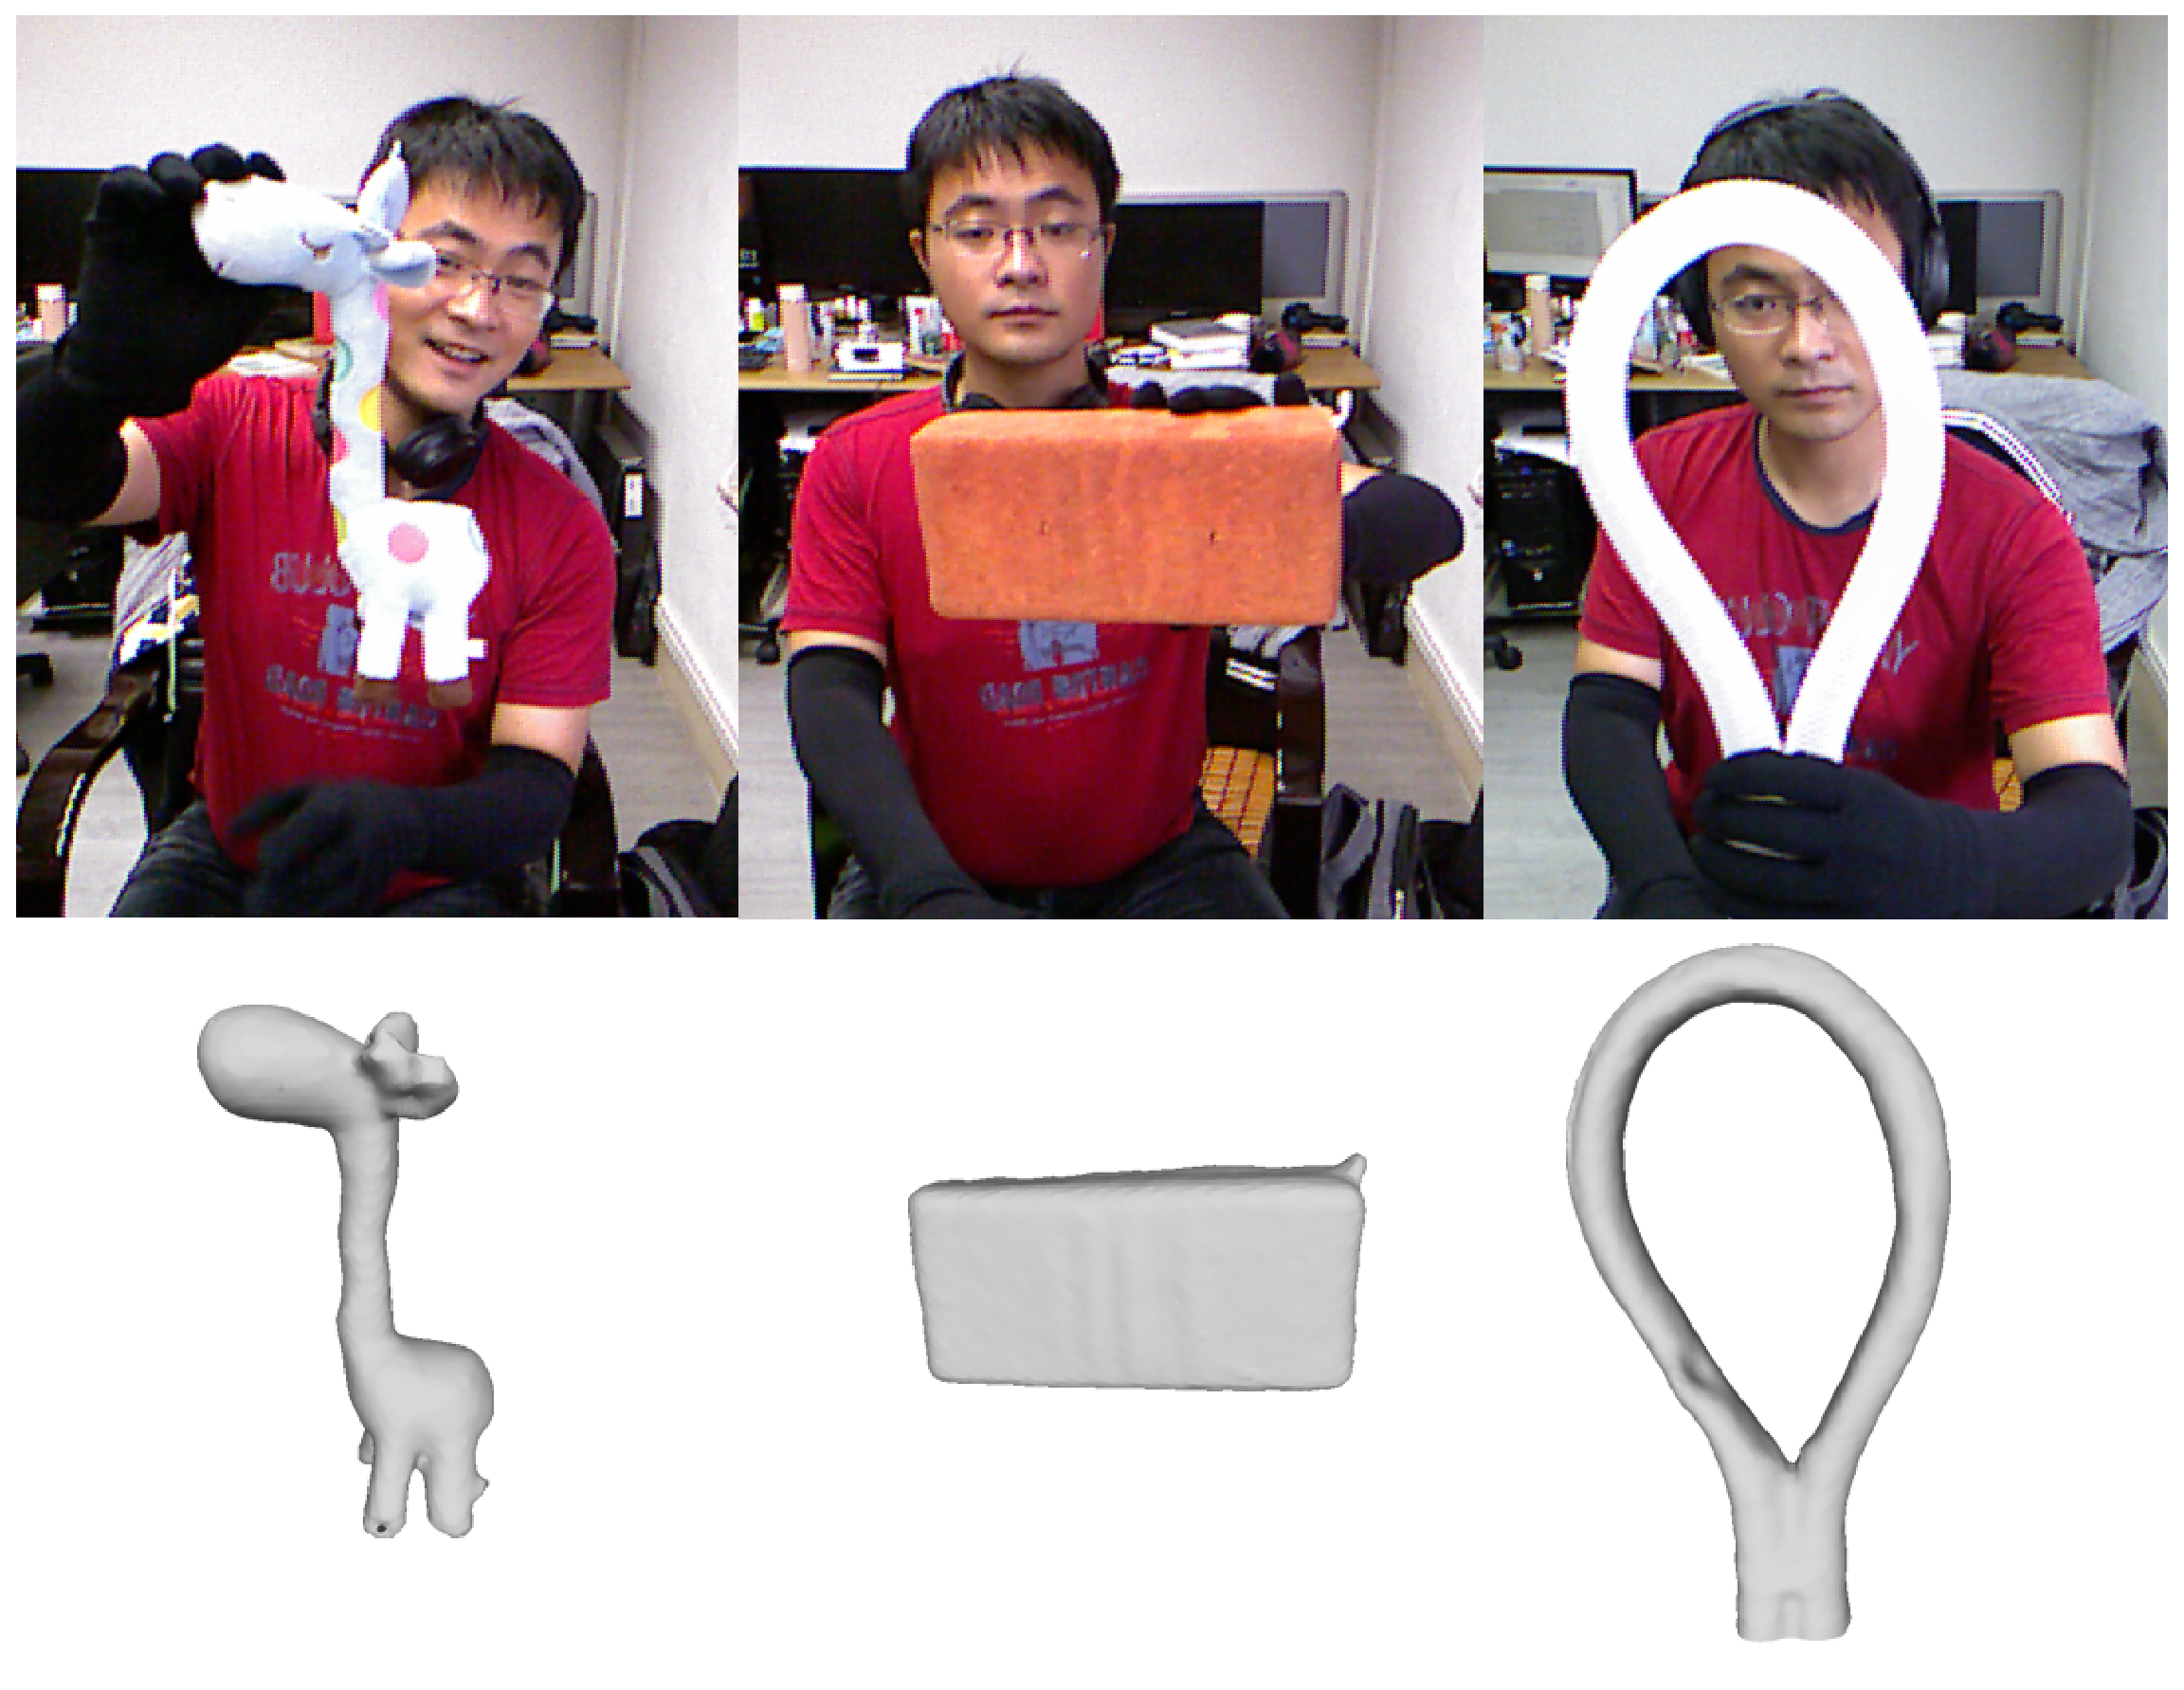
\includegraphics[width=0.9\textwidth]{./Pictures/static_mesh.eps}
    \caption{采集静态模型}
    \label{static_model}
\end{figure}

\section{基于深度相机的三维重建}
对于现实世界中存在的物体,其三维模型通常可以通过CAD软件建模或者借助扫描设备重建。
本文所使用的模型均借助深度相机重建。

深度相机是一种可以获取深度信息的设备,即能够测量物体表面距离相机的距离。
如同章节\ref{range_finding}所说,现在较为流行的三维测距技术有飞行时间、三角测距和结构光。
本文采用的是Microsoft生成的Kinect一代,这是一台基于结构光技术的深度相机。
Kinect除了能够获得RGB图像外,还能获得深度图像。
深度图像的每个像素记录的是物体表面距离相机的距离,
利用透视原理,可以推算出物体表面和相机的相对位置。
三维重建算法就可以通过扫描过程中获取的深度信息重建出物体的几何信息,获得三维模型。
本文采用的是KinectFusion算法\cite{izadi2011kinectfusion},
能够实时的借助深度相机重建三维模型。
KinectFusion算法\cite{izadi2011kinectfusion}以深度视频(由深度图像组成的图像流)为输入。
对于每一帧,会计算物体和相机的相对位置(物体在相机坐标系中的位置)
以及相机在世界坐标系(通常是第一帧的相机坐标)中的位置,
并将每一帧获得的数据融合到一个统一的模型坐标系中,从而得到三维模型。




\chapter{基于深度相机模型形变捕捉}
要构建模型的形变子空间,除了静态三维模型,
还需要一些形变后的模型,即形变关键帧作为输入。
本章描述了一个以静态模型和深度视频为输入的形变捕捉算法。
在捕捉步骤中,操作者会带着特定颜色的手套,在深度相机前摆弄物体,使得物体发生形变。
该算法会优化模型的形变参数,使得模型的形状和相机采集的物体形状尽量吻合,
从而得到形变后的模型。
本文会从捕捉到的形变中选取若干成为形变关键帧,作为形变子空间构建的输入。
本章接下来就会阐述该算法的技术细节。

\section{基于手部信息的模型初始位姿估计}

 类似于三维重建步骤中的相机位姿估计,
 在形变步骤中,对于每一帧深度图像,本文仅计算模型和上一帧的相对形变。
 因此,在捕捉形变之前,需要得知模型的初始位置。
 在本文的形变捕捉流程中,操作者需要用手持物。
 所以物体必然位于手的附近,所以本文设计了一个借助手部信息确定模型的初始位置与朝向的算法。
 本位所采用的确定物体初始位姿的算法可主要分为三个步骤:分割手部点云、分割物体点云、模型对齐。
 本节接下来就会详细描述这一流程。

\subsection{手部点云分割}
由于本文是借助手部点云的位置寻找物体的点云,
所以需要在输入的点云中分割出属于手的部分。
本章就将描述一种基于RGBD图像的点云分割算法。
\begin{figure}[h]
    \centering
    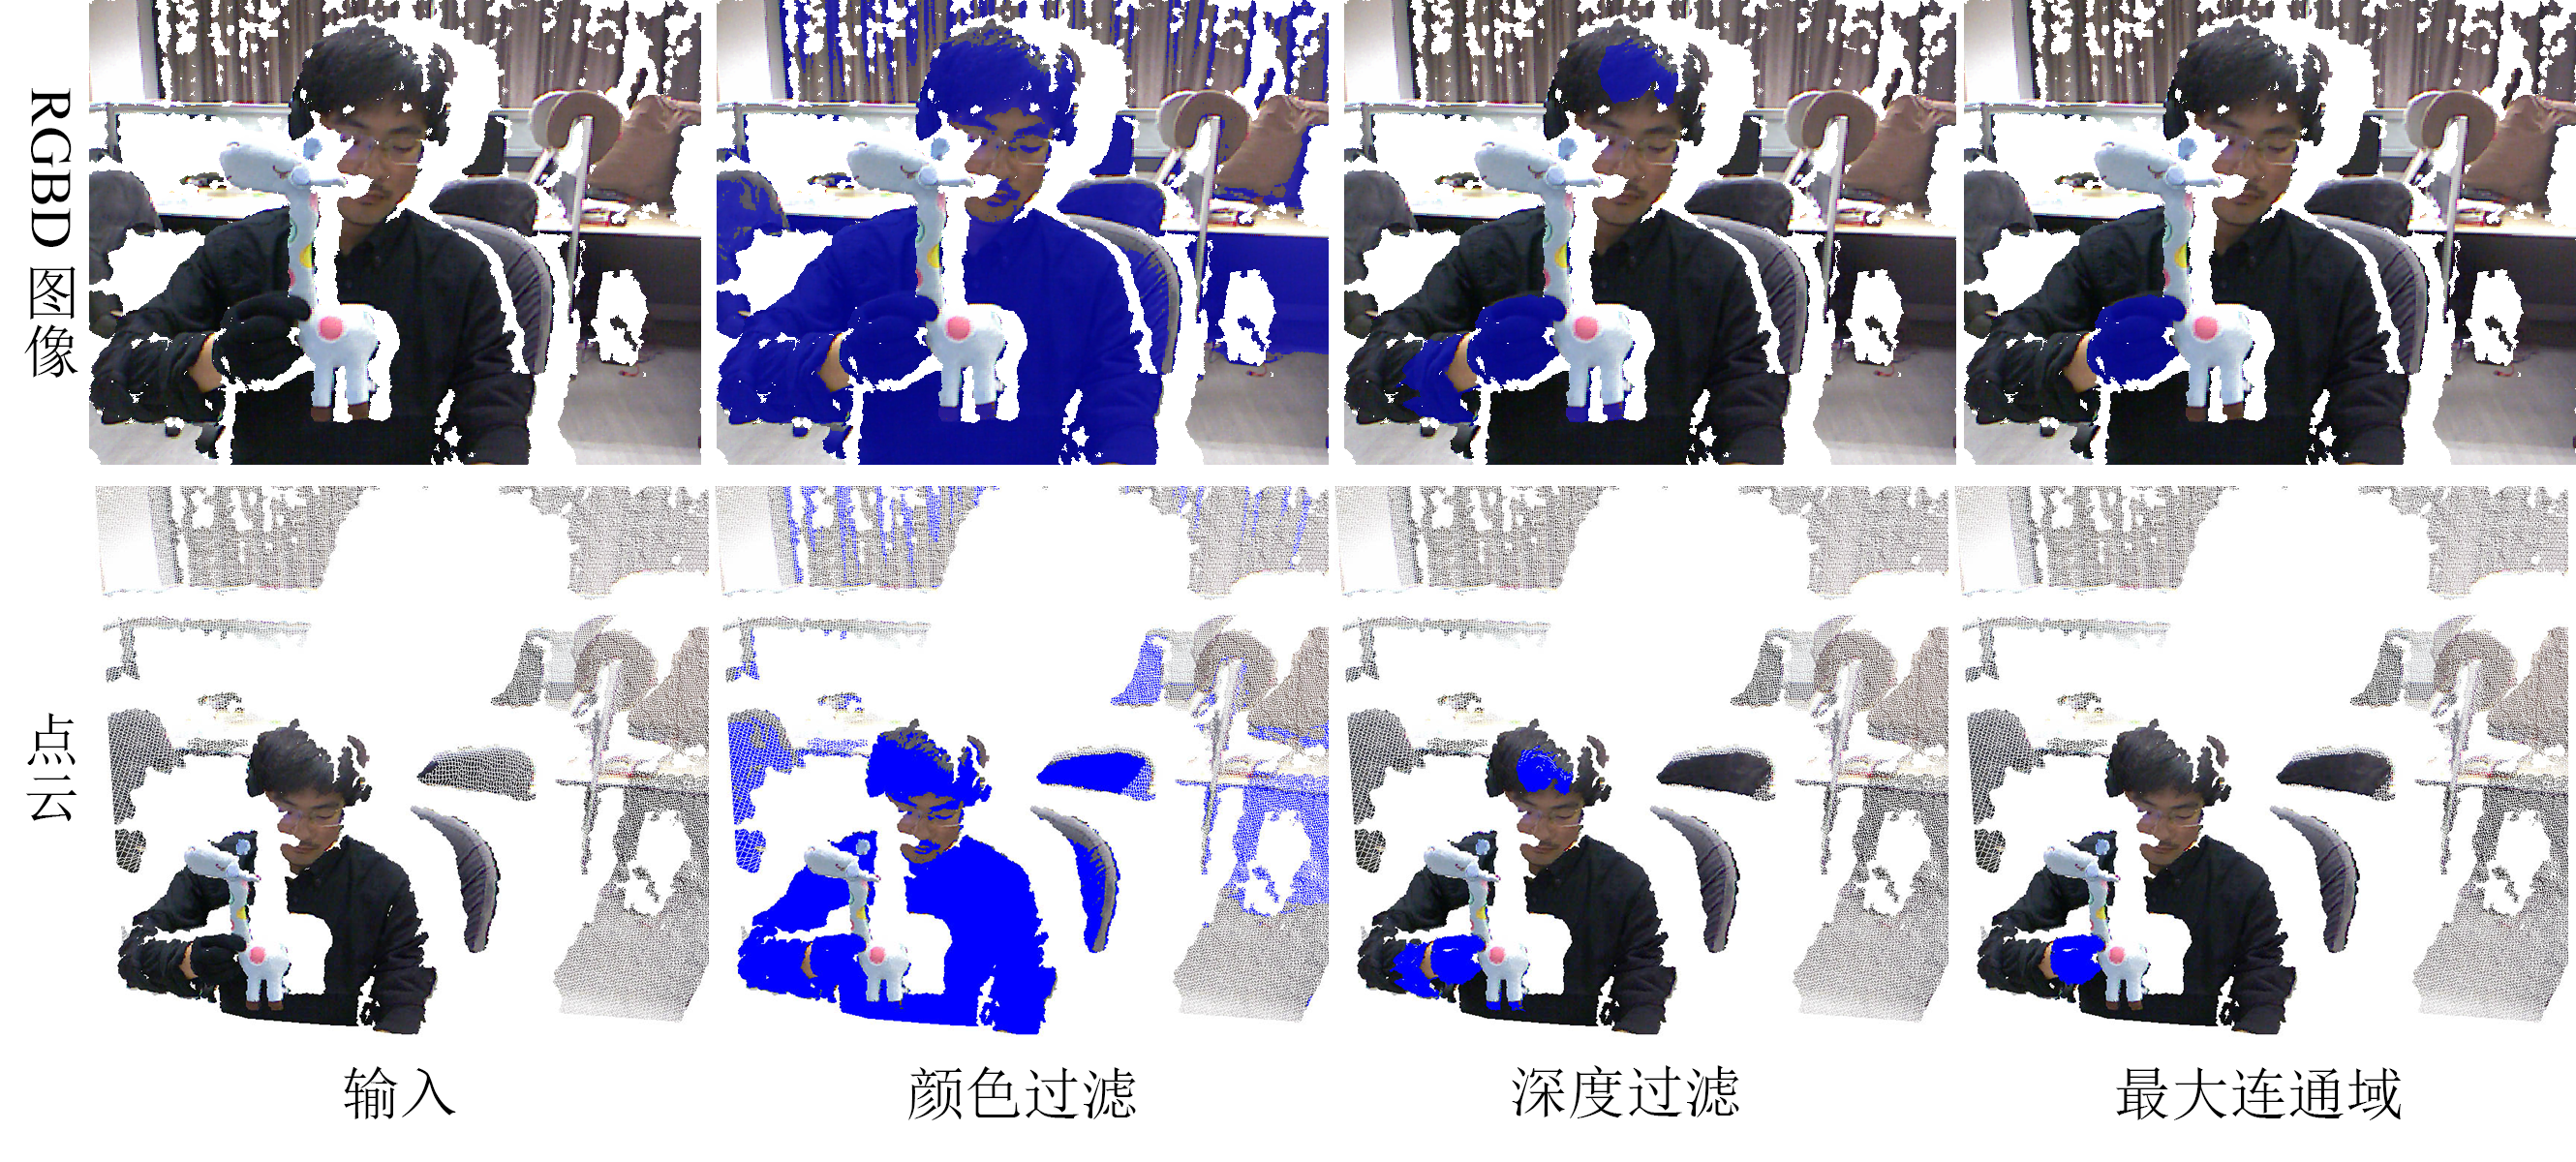
\includegraphics[width = \textwidth]{./Pictures/FindingHand.png}
    \caption{手部点云分割流程}
    \label{finding_hand}
\end{figure}
分割手部点云阶段的输入是RGBD图像,输出为手部的像素坐标的集合。
RGBD图像即除了RGB三个颜色通道外,还有一个深度通道
记录了对应点距离相机的距离,可以理解为RGB图像加上深度图像。
Kinect分别通过色彩传感器和深度传感器获得RGB图像和深度图像,
由于两个传感器的相对位置被事先标定过,
所以Kinect的SDK提供了将RGB图像映射到深度图像的接口,
映射后的RGB图像的像素和深度图像的像素一一对应。
图\ref{finding_hand}第一行的第一张图就是映射到相应深度图位置后的RGB图像。
本文中提到的RGB图像均默认指映射后的RGB图像。

在操作物体时,操作者会带上特定颜色的手套,以对相应的数据做特殊处理。
找出手部数据的主要目的是在后续的形变捕捉步骤中过滤掉所有手部的深度信息,
因为手部的深度信息对于形变捕捉是很大的噪声。
在形变捕捉的前置阶段——初始位置阶段,
手部信息也作为辅助信息用于确定物体的初始位姿
如图\ref{finding_hand}和算法\ref{alg_seg_hand}所示,
分割手部点云阶段可主要分为颜色过滤、深度过滤、寻找最大连通域三个步骤。
图\ref{finding_hand}的第一行的图片中被标记为蓝色的部分是每个步骤确定的手的位置,
第二行的图片是对应的点云。
\begin{algorithm}
    \fangsong
    \caption{分割手部点云}
    \label{alg_seg_hand}
    \begin{algorithmic}[1]
        \Require RGB图像$\mathbf{C_i}$,深度图像$\mathbf{D_i}$
        \Ensure 手部像素集合$\mathbf{S_{hand}}$
        \Procedure{GetHandPixels}{$\mathbf{C_i}$, $\mathbf{D_i}$}
            %\State $\mathbf{V_i} \gets$ \Call{DepthToVertex}{$\mathbf{D_i}$}
            \State $\mathbf{S_{hand}} \gets$ \Call{ColorFilter}{$\mathbf{C_i}$}
            \State $\mathbf{S_{hand}} \gets$ \Call{DepthFilter}{$\mathbf{D_i}$, $\mathbf{S_{hand}}$}
            \State $\mathbf{S_{hand}} \gets$ \Call{LargestConnectedDomain}{$\mathbf{S_{hand}}$}
        \EndProcedure
    \end{algorithmic}
\end{algorithm}

首先,本文会进行颜色过滤步骤,筛选出输入图像中与手套颜色相近的像素点。
算法\ref{alg_cfilter}描述了颜色过滤的流程。
其中$\mathbf{C_{hand}}$和$thd_{color}$分别是预先设定的手套颜色的集合和颜色距离阈值。
%本文的实验中$thd_{color}$的值设为50。
在该步骤中,会遍RGB图像的每一个像素。
如果该像素的颜色和$\mathbf{C_{hand}}$中的任何颜色相近,
即在RGB颜色空间中与相应颜色距离小于$thd_{color}$的像素,
就会被认为可能是手部的像素,并入待选集合中。
颜色过滤的记过如图\ref{finding_hand}中第二列所示。
从图中可以看出,颜色过滤会将图像背景中大量颜色与手套相近的像素判定为手部像素。
所以,如果要借助手的位置确定物体的位置,还需要进一步的筛除背景中多余的像素。
\begin{algorithm}
    \fangsong
    \caption{颜色过滤}
    \label{alg_cfilter}
    \begin{algorithmic}[1]
        \Require RGB图像$\mathbf{C_i}$
        \Ensure 像素点集合$\mathbf{S}$
        \Function {ColorFilter}{$\mathbf{C_i}$}
            %\State $\mathbf{S} \gets \varnothing$
            \For {$\forall\mathbf{u} \in$ \Call{PixelDomain}{$\mathbf{C_i}$}}
                \For {$\forall\mathbf{c} \in \mathbf{C_{hand}}$}
                    \If{$\|\mathbf{C_i}(u) - \mathbf{c}\| \leq thd_{color}$}
                    \State $\mathbf{S} \gets \mathbf{S} \bigcup \{\mathbf{c}\}$
                    \EndIf
                \EndFor
            \EndFor 
            \State \Return $\mathbf{S}$
        \EndFunction
    \end{algorithmic}
\end{algorithm}

在颜色过滤后,本文会执行深度过滤步骤,即只保留深度最小像素点。
从图\ref{finding_hand}中可以看出,在操作者手持物体操作的过程中,
握着物体的手总是位于最前方。
%在这种特定的场景中,本文默认手部的像素点必在深度值最小的那部分像素之中。
算法\ref{alg_dfilter}描述了深度过滤的流程。
其中,$d_{range}$是预先设定的筛选深度范围,%在本文的实验中设为150毫米。
$d_{min}$是集合中深度最小的像素的深度值。
然后遍历集合中的每个像素,仅保留深度值小于$d_{min}+d_{range}$的像素。
深度过滤的结果如图\ref{finding_hand}第三列所示。
% \begin{algorithm}
%     \fangsong
%     \caption{深度图像转点云}
%     \label{alg_d2v}
%     \begin{algorithmic}
%         \Require 深度图像$\mathbf{D_i}$
%         \Ensure 点云$\mathbf{V_i}$
%         \Function {DepthToVertex}{$D_i$}
%             \For{$\forall \mathbf{u} \in$ \Call{PixelDomain}{$\mathbf{D_i}$}}
%                 \State $\mathbf{V_i(u)}=\mathbf{D_i}(\mathbf{u})\mathbf{K}^-1[\mathbf{u},1]$
%             \EndFor
%             \State \Return $\mathbf{V_i}$
%         \EndFunction
%     \end{algorithmic}
% \end{algorithm}
\begin{algorithm}
    \fangsong
    \caption{深度过滤}
    \label{alg_dfilter}
    \begin{algorithmic}[1]
        \Require 深度图像$\mathbf{D_i}$, 像素点集合$\mathbf{S_{in}}$
        \Ensure 像素点集合$\mathbf{S_{out}}$
        \Function {DepthFilter}{$\mathbf{D_i}$, $\mathbf{S_{in}}$}
            %\State $\mathbf{Set_{out}} \gets \mathbf{Set_{int}}$
            \State $d_{min} \gets$ \Call{Min}{$\mathbf{D_i}$}
            \For {$\forall \mathbf{u} \in \mathbf{S_{in}}$}
                \If {$\mathbf{D_i}(\mathbf{u}) < d_{min}$ or $\mathbf{D_i}(\mathbf{u}) > d_{min} + d_{range}$}
                    %\State $\mathbf{Set_out} \gets \mathbf{S} - \{u\}$
                    \State $\mathbf{S_{out}} \gets \mathbf{S_{out}} \bigcup \{\mathbf{u}\}$
                \EndIf
            \EndFor
            \State \Return $\mathbf{S_{out}}$
        \EndFunction
    \end{algorithmic}
\end{algorithm}
\begin{algorithm}
    \fangsong
    \caption{获取最大连通域}
    \label{alg_lcd}
    \begin{algorithmic}[1]
        \Require 像素点集合$\mathbf{S}$
        \Ensure 最大连通域$\mathbf{LCD}$
        \Function {LargestConnectedDomain}{$\mathbf{S}$}
            %\State $\mathbf{LCD} \gets \varnothing$
            \For{$\forall \mathbf{u} \in \mathbf{S}$}
                \If{$\mathbf{u}$ not checked}
                    \State $\mathbf{CD} \gets$ \Call{GetConnectedDomain}{$\mathbf{S}$, $\mathbf{u}$}
                    \If{$|\mathbf{CD}| > |\mathbf{LCD}|$}
                        \State $\mathbf{LCD} \gets  \mathbf{CD}$
                    \EndIf
                \EndIf
            \EndFor
            \State \Return $\mathbf{LCD}$
        \EndFunction
        \Function {GetConnectedDomain}{$\mathbf{S}$, $\mathbf{u}$}
            %\State $Q \gets$ \Call{EmptyQueue}{},$\mathbf{CD} \gets \varnothing$
            \State \Call{QueuePush}{$Q$, $\mathbf{u}$}
            \State Set $\mathbf{u}$ as checked
            \While{$Q$ not empty}
                \State $\mathbf{u_i} \gets$ \Call{QueuePop}{$Q$}
                \State $\mathbf{CD} \gets \mathbf{CD} \bigcup \{\mathbf{u_i}\}$
                \For{$\forall \mathbf{u_{neighbor}} \in$ \Call{NeighborPixel}{$\mathbf{u_i}$}}
                    \If{$\mathbf{u_{neighbor}}$ not checked}
                        \State \Call{QueuePush}{$Q$, $\mathbf{u_{neighbor}}$}
                        \State Set $\mathbf{u_{neighbor}}$ as checked
                    \EndIf
                \EndFor
            \EndWhile
            \State \Return $\mathbf{CD}$
        \EndFunction
    \end{algorithmic}
\end{algorithm}
在深度过滤后,本文将在已经判定为手部的像素集合中找到其在图像空间中最大连通域,
进一步去除零散的像素点。
以带黑色手套为例,这些被误判的像素点可能是物体上阴影所在的部分,
也可能是身体靠近物体的部分。
这些被误判的区域会影响物体位置的估计。
在实验的过程中可以发现,在深度过滤之后,真正的手部在图像中,
大都落在已判定区域中的最大连通域里。
所以本文在深度过滤的结果中寻找图像空间中的最大连通域,作为最终的手部区域。
算法\ref{alg_lcd}描述了该步骤的流程。
GetConnectedDomain函数采用了广度优先搜索的方式计算与指定像素位置$\mathbf{u}$
相连的连通域;
LargestConnectedDomain函数遍历了集合中所有的连通域,并找到其中最大的连通域。
最终分割出的手部点云如图\ref{finding_hand}第四列所示。

在上述步骤中,颜色过滤和深度过滤各像素位置的计算是互相独立的,可用GPU并行加速。
其中颜色过滤在实现时与RGB图映射到深度图的步骤在同一个CUDA Kernel中实现。
最大连通域的计算需要根据各像素的邻接关系,不便于大规模并行。
且经由之前的筛选,该步骤需要遍历的像素已大为减少,所以在CPU上可以很快的完成。


\subsection{物体点云分割}

\subsection{模型对齐}

\section{基于深度视频的形变捕捉}
\subsection{形变的参数化描述}
\subsection{形变参数优化}

\section{本章小结}

\chapter{基于深度视频的形变关键帧获取}
要构建模型的形变子空间,除了静态三维模型,
还需要一些形变后的模型,即形变关键帧作为输入。
本章描述了一个以静态模型和深度视频为输入的形变捕捉算法。
在捕捉步骤中,操作者会带着特定颜色的手套,在深度相机前摆弄物体,使得物体发生形变。
该算法会优化模型的形变参数,使得模型的形状和相机采集的物体形状尽量吻合,
从而得到形变后的模型。
本文会从捕捉到的形变中选取若干成为形变关键帧,作为形变子空间构建的输入。
本章接下来就会阐述该算法的技术细节。
\section{网格形变的描述}
本文采用基于双四元数(Dual Quaternions)的形变图(Deformation Graph)描述网格模型的形变,
形变捕捉步骤就是通过优化形变图的参数使得模型的形状尽可能贴近相机采集的物体形状。
本节接下来将详细介绍本文描述网格形变的方法。
\subsection{双四元数}
本小节将提供一个双四元数的简介。
简介主要关注四元数的定义与基本性质,以及本文所需要的一些特性与应用,
会略过数学证明的内容。
如果想进一步了解有关双四元数的细节,
可以自行查阅相关资料\cite{mccarthy1990introduction}\cite{kavan2006dual}。

双四元数是一种描述三维变换的工具,可以看做是四元数的扩展。
四元数是一种在计算机图形学中被广泛应用的描述三维空间中旋转的工具,
本节默认读者熟悉四元数的性质与应用,再此不多做介绍。
相较于常规的四元数,双四元数不是那么常见。
但与四元数只能描述旋转不同,双四元数可以描述三维空间中的刚体变换,
即其所描述的三维变化不仅包含旋转还包含了平移。

双四元数可看成元素为二元数(dual number)的四元数。与复数相似,二元数是实数的推广。
一个二元数$\hat{a}$可以被写成$\hat{a} = a_0 + \varepsilon a_{\varepsilon}$,
其中$a_0$是非二元部,$a_{\varepsilon}$是二元部,
$\varepsilon$是二元单元,${\varepsilon}^2=0$。
二元数的共轭与复数相似$\bar{\hat{a}} = a_0 + a_{\varepsilon}$。
二元数数的乘法可以展开为
$(a_0+\varepsilon a_{\varepsilon})(b_0 + \varepsilon b_{\varepsilon})=
 a_0b_0 + \varepsilon (a_0b_{\varepsilon} + a_{\varepsilon}b_0)$。
二元数的逆可以表示为
\begin{equation}
    \hat{a}^{-1}=\frac{1}{a_0+\varepsilon a_{\varepsilon}}
    =\frac{1}{a_0}-\varepsilon \frac{a_{\varepsilon}}{a^2_0}
\end{equation}

一个双四元数$\hat{\bm{q}}$可以被写成
$\hat{\bm{q}}=\hat{w}+i\hat{x}+j\hat{y}+k\hat{z}$,
其中$\hat{w}$为标量部分(二元数标量),
$(\hat{x},\hat{y},\hat{z})$为向量部分(二元数向量),
$i$、$j$、$k$是四元数单位。
双四元数也可以被写成八元组形式或两个四元数的形式,
$\hat{\bm{q}}=\bm{q_0}+\varepsilon \bm{q_{\varepsilon}}$,
而双四元数的共轭被定义为将两个四元数部分分别取共轭,
$\hat{\bm{q}}^*=\bm{q_0}^*+\varepsilon \bm{q_{\varepsilon}}^*$。
双四元数的范数$\|\hat{\bm{q}}\|=
              \sqrt{\hat{\bm{q}}^* \hat{\bm{q}}} =\sqrt{\hat{\bm{q}} \hat{\bm{q}}^*}$
可被展开为
\begin{equation}
    \label{eq_norm_dq}
    \|\hat{\bm{q}}\| = 
    \sqrt{\hat{\bm{q}}^* \hat{\bm{q}}} = 
    \|\bm{q_0}\| + 
    \varepsilon \frac{\langle \bm{q_0}, \bm{q_{\varepsilon}}\rangle}{\| \bm{q_0} \|} 
\end{equation}
双四元数的范数满足性质
$\|\hat{\bm{p}}\hat{\bm{q}}\| = \|\hat{\bm{p}}\| \|\hat{\bm{q}}\|$。
根据公式\ref{eq_norm_dq}可知,
双四元数的逆$\hat{\bm{q}}^-1= \frac{\hat{\bm{q}}^*}{\|\hat{\bm{q}}\|}$
当且仅当$\bm{q_0} \neq 0$时存在。
范数为1的双四元数被称为单位双四元数。
根据公式\ref{eq_norm_dq}可知,当且仅当$\|\bm{q_0}\|=1$且
$\langle \bm{q_0}, \bm{q_{\varepsilon}}\rangle = 0$
时,双四元数$\hat{\bm{q}}=\bm{q_0}+\varepsilon \bm{q_{\varepsilon}}$为单位双四元数。
有此可以看出,单位双四元数并不总是可逆的。
所以双四元数满足结合律和分配率但不满足交换律。

当二元部$\bm{q_{\varepsilon}}=\bm{0}$时,单位双四元数可以表示三维空间中的旋转。
对于三维向量$(v_0,v_1,v_2)$可以构造对应的双四元数
$\hat{\bm{v}}=1 + \varepsilon (v_0i + v_1j + v_2k)$。
向量$(v_0,v_1,v_2)$关于单位双四元数$\hat{\bm{q}}$的旋转可以被表示为
$\hat{\bm{q}} \hat{\bm{v}} \bar{\hat{\bm{q}}^*}$。
可以证明,当$\bm{q_{\varepsilon}}=\bm{0}$时,$\hat{\bm{q}}=\bm{q_0}$,
所以$\hat{\bm{q}} \hat{\bm{v}} \bar{\hat{\bm{q}}^*}$可被简化为
\begin{equation}
    \bm{q_0}
    (
        1 + \varepsilon (v_0i + v_1j + v_2k)
    )
    \bm{q_9}^*
    =
    1 + \varepsilon \bm{q_0}(v_0i + v_1j + v_2k)\bm{q_0}^*
\end{equation}
可以看出$\bm{q_0}(v_0i + v_1j + v_2k)\bm{q_0}^*$即为由常规四元数定义的旋转。
此外,当$\bm{q_0} = 1$时,双四元数可以表示三维空间中的平移变换。
双四元数$\hat{\bm{t}} = 1 + \frac{\varepsilon}{2} (t_0i + t_1j + t_2k)$
能够表示向量$(t_0,t_1,t_2)$所描述的平移变换。
经计算不难得知,
$\hat{\bm{t}} \hat{\bm{v}} \bar{\hat{\bm{t}}^*}$可被简化为
$
1 + \varepsilon (
        (v_0 + t_0)i +
        (v_1 + t_1)j +
        (v_2 + t_2)k
    )
$
刚体变换时旋转与平移的结合,而双四元数表示变换可以通过双四元数乘法叠加。
若用单位四元数$\bm{q_0}$描述旋转,
用单位双四元数$1 + \frac{\varepsilon}{2} (t_0i + t_1j + t_2k)$描述平移,
则该刚体变换对应的四元数为
\begin{equation}
    \label{eq_dq_rt}
    (1 + \frac{\varepsilon}{2} (t_0i + t_1j + t_2k))
    \bm{q_0}
    =
    \bm{q_0} + \frac{\varepsilon}{2} (t_0i + t_1j + t_2k)\bm{q_0}
\end{equation}
可以证明,公式\ref{eq_dq_rt}的结果一定是单位双四元数,
且所有单位双四元数都可以写成如上形式。
如同$3 \times 3$的旋转矩阵可以与四元数互相转换,
$4 \times 4$的刚体变换矩阵也可以与双四元数互相转换。

利用双四元数,可以方便的进行刚体变换的插值运算。
Kavan等人\cite{kavan2006dual}提出了双四元数线性混合
(DLB  Dual quaternion Linear Blending)用于
两个及两个以上的双四元数的插值
\begin{equation}
    DLB(\bm{w},\hat{\bm{q_1}},\ldots,\hat{\bm{q_n}}) = 
    \frac{
            w_1\hat{\bm{q_1}} + \ldots + w_n\hat{\bm{q_n}}
        }
        {
            \| w_1\hat{\bm{q_1}} + \ldots + w_n\hat{\bm{q_n}}\|
        }
\end{equation}
$DLB$满足以下几个性质:
\begin{enumerate}
    \item  $DLB$的返回值永远是刚体变换。
    \item  $DLB$具有坐标不变性。
           对于任何单位双四元数$\hat{\bm{r}}$,满足
           \begin{equation}
                DLB(\bm{w},\hat{\bm{r}}\hat{\bm{q_1}}\hat{\bm{r}}^*,
                \ldots , 
                \hat{\bm{r}}\hat{\bm{q_n}}\hat{\bm{r}}^*)
                =
                \hat{\bm{r}}DLB(\bm{w},\hat{\bm{q_1}},\ldots,\hat{\bm{q_n}})\hat{\bm{r}}^*
           \end{equation}
    \item  当$DLB$作用于两个刚体变换时,它会在二者间的最短路径上插值。
\end{enumerate}
本文就是采用$DLB$进行刚体变换的插值。
关于以上性质的证明,
可以查阅Kavan等人\cite{kavan2006dual}的论文。

\subsection{基于双四元数的形变图}
本文采用基于双四元数的形变图描述网格图形的形变。
形变图(Deformation Graph)\cite{sumner2007embedded}
是一种被广泛应用的通用的描述形变的方法,通常用于模型的形状编辑。
形变图是一种特殊的图结构,由节点集合$\bm{Node}$和边集合$\bm{Edge}$组成。
$\bm{Node}$中的每个节点$node_i = \{\bm{vn_i}, \hat{\bm{q}}_i\}$
记录了节点在未形变时的位置$\bm{vn_i}$以及该节点在模型空间中发生的刚体变换$\hat{\bm{q}}_i$。
$\bm{Edge}$中的边$edge_{ij}$连接了$node_i$与$node_{j}$。
相连的节点在优化的过程中会互相约束,
以保证形变过程中能够保持模型的局部特征。

原始的形变图中,图中的节点用旋转矩阵和平移向量描述该节点的刚体变换。
本文借鉴了Dynamic Fusion\cite{newcombe2015dynamicfusion}中的形变框架Warp Field,
用双四元数$\hat{\bm{q}}$描述节点的刚体变换。
相较于变换矩阵,双四元数有以下优点:
\begin{enumerate}
    \item   双四元数拥有更少的参数。
            旋转矩阵和平移向量共有$9+3=12$个参数,每个节点需12个参数。
            而一个双四元数共有8个变量,使整个形变图的控制参数减少了三分之一,
            使得需要优化的变量更少。
    \item   不需要额外约束确保旋转矩阵不含缩放与剪切变换。
            对于$3 \times 3$的变换矩阵所定义三维变换除了旋转外,
            还可能包含缩放与剪切。所以在原始的形变图模的优化中,
            会再能量函数中添加约束使得优化后的矩阵仍然是旋转矩阵。
            但双四元数所描述的变换必然是刚体变换,无需添加额外的软约束。
    \item   双四元数可通过$DLB$直接插值。
            变换矩阵无法直接插值,
            原始的形变图是通过计算各节点与模型顶点在形变前的相对位置估算出顶点的当前位置,
            然后再对各顶点估算出的顶点位置做线性插值,最终得到顶点在形变后的位置。
            这一过程十分繁琐。
            而四元数则可以直接进行对刚体变换插值。
            所以对于模型上的顶点,可以直接计算出该顶点需要的刚体变换,
            使得计算顶点位置的步骤更为简洁高效。
            而且,如上一小节所说,利用$DLB$进行双四元数的插值具有良好的性质,
            通过插值得到的形变结果也较为自然。
\end{enumerate}

在基于双四元数的形变图构建完成后,
就可以利用双四元数插值计算出空间中任意一点刚体变换。
由此可以定义一个映射$G:\mathbb{R}^3\rightarrow \bm{SE}(3)$。
其中$\bm{SE}(3)$为三维欧氏群,可看做所有三维空间中的刚体变换矩阵的集合。
本文对函数$G$做如下定义:
\begin{equation}
    G(\bm{x})\equiv Q2T(
        \frac
        {\sum_{node_k \in \bm{GN}(x)}w(\bm{x},\bm{vn_k}) \hat{\bm{q_k}}}
        {\| \sum_{node_k \in \bm{GN}(x)}w(\bm{x},\bm{vn_k}) \hat{\bm{q_k}} \|}
    )
\end{equation}
可以看出$\frac
        {\sum_{node_k \in \bm{GN}(x)}w(\bm{x},\bm{vn_k}) \hat{\bm{q_k}}}
        {\| \sum_{node_k \in \bm{GN}(x)}w(\bm{x},\bm{vn_k}) \hat{\bm{q_k}} \|}$
就是以$w(\bm{x},\bm{vn_k})$为权重,利用$DLB$对相应的节点的双四元数进行插值,
得到描述$\bm{x}$处所需刚体变换的双四元数,而$Q2T$是将双四元数转换为相应刚体变换矩阵的函数。
其中$\bm{GN}(x)$包含了$\bm{Node}$中距离$x$最近的$k$个节点,
$ w(\bm{x},\bm{vn_k})$为节点$node_k$在位置$\bm{x}$出插值的权重
\begin{equation}
    w(\bm{x},\bm{vn}) = e^{-\frac{\| \bm{vn} - \bm{x} \|}{2r_G^2}}
\end{equation}
$\bm{x}$与$\bm{vn}$越接近权重越大。
$r_G$为构建形变图时节点的距离,定义了图中节点的离散程度。

可以看出基于双四元数形变图定义了空间中的一个场,场中每个位置的刚体变换会受附近节点的影响。
所以Dynamic Fusion中将这种用双四元数描述的形变框架称为Warp Field。
为了便于描述,本文之后提到的形变图均为基于双四元数的形变图。

\subsection{形变图的构建}  
对于给定的网格模型,本文会自动构建与之对应的形变图。
形变图的节点会尽可能均匀的分布在模型的表面,并用边连接相邻的节点。
算法\ref{alg_build_graph}描述了形变图构建的流程。
形变图的构建可主要分为三个步骤:
生成节点、生成边、记录每个顶点的k最近邻节点。
\begin{algorithm}
    %\fangson
    \caption{形变图构建}
    \label{alg_build_graph}
    \begin{algorithmic}[1]
        \Procedure{BuildGraph}{$\bm{V_{mesh}}$,$r_G$,$k_e$,$k_v$}
            \State build KD Tree from $\bm{V_{mesh}}$
            \State $\bm{Node} \gets$ \Call{GenerateNodes}{$\bm{V_{mesh}}$,$r_G$}
            \State build KD Tree from $\bm{Node}$
            \State $\bm{Edge} \gets$ \Call{GenerateEdges}{$\bm{Node}$,$k_e$}
            \State $\bm{GN} \gets$ \Call{FindKnnNodesForVertex}{$\bm{Node}$,$\bm{V_{mesh}}$, $k_v$}
        \EndProcedure
    \end{algorithmic}
\end{algorithm} 

首先,本文会在网格模型的表面均匀的生成形变节点。
可以看出形变节点分布的密度可通过参数$r_G$控制,
边的数目可用阐述$k_e$控制,
控制每个顶点的节点的个数可通过$k_v$控制。
算法\ref{alg_gen_nodes}描述了该步骤的实现流程。
构建形变图的的第一步是在模型表面生成均匀分布的形变节点。
该步骤的输入时模型中的所有顶点$\bm{V_{mesh}}$与节点间的最大距离$r_G$。
本文会从模型中所有顶点所在的位置中采样,并保证生成的任意两个节点的距离不小于$r_G$。
在这一步中,本文会维护一个未被任何节点覆盖的顶点的集合
\begin{equation}
    \bm{V_{uncovered}}  = \{\bm{v} \in \bm{V_{mesh}} \quad |
    \quad \forall node_i \in \bm{Node}: \| \bm{vn_i} - \bm{v}\| > r_G\}
\end{equation}
在循环开始前,$\bm{V_{uncovered}}$包含$\bm{V_{mesh}}$中的顶点。
在每一次循环中,在$V_{uncovered}$里随机挑选一个顶点$\bm{v_r}$,作为新的节点。
然后找出所有与该节点的距离小于$r_G$的模顶点,被称为已覆盖顶点,将其从$\bm{V_{uncovered}}$中剔除。
为了提高查找已覆盖顶点的效率,
本文会在开始生成节点之前,以模型中所有顶点的位置为元素构建一个KD Tree。
这样形变图节点附近的模型顶点通过KD Tree进行快速的查找。
上述过程会不断重复,直到$\bm{V_{uncovered}}$中的顶点全部被剔除。
\begin{algorithm}
    %\fangsong
    \caption{生成形变图节点}
    \label{alg_gen_nodes}
    \begin{algorithmic}[1]
        \Function{GenerateNodes}{$\bm{V_{mesh}}$,$r_G$}
        %\State $KDTree \gets$ build KD-Tree with all vertices in $V_{mesh}$
        \State $\bm{V_{uncovered}} = \bm{V_{mesh}}$
        \While{$\bm{V_{uncovered}} \neq \varnothing $}
            \State $\bm{v_r} \gets$ randomly select a vertex in $V_{uncovered}$
            \State $node.\bm{vn} \gets \bm{v_r}$
            \State $\bm{Node} \gets \bm{Node} \bigcup \{node\}$
            \State $\bm{V_{uncovered}} \gets \bm{V_{uncovered}} - 
                    \{\bm{v} \in \bm{V_{uncovered}} \quad | \quad 
                    \|\bm{v} - \bm{v_r}\| \leq r_G\}$
        \EndWhile
        \State \Return $\bm{Node}$
    \EndFunction
    \end{algorithmic}
\end{algorithm} 

在生成了形变图之后,本文会用边连接相邻的节点。
本文用k最近邻的策略进行边的构建,为了提高k最近邻查找的速度,
本文在生成了形变图节点后,以节点的位置为元素构建一棵KD Tree。
算法\ref{alg_gen_edges}描述了生成形变图边的过程:
对于图中的每个节点$node_i$,利用KD Tree找出离它$k_e$个节点。
对于每个找到的近邻节点$node_j$,构建一条从$node_i$到$node_j$的边。
可以看出,形变图中的边是单向边,所以形变图是一个单向图。
单向图的边对于模型顶点位置的插值计算并无影响,
但它在形变参数优化的过程中对于模型的平滑性有着重要的作用。
图\ref{build_graph}为$k_e=6$,$k_v=4$时构建出的形变图。
\begin{figure}[]
    \centering
    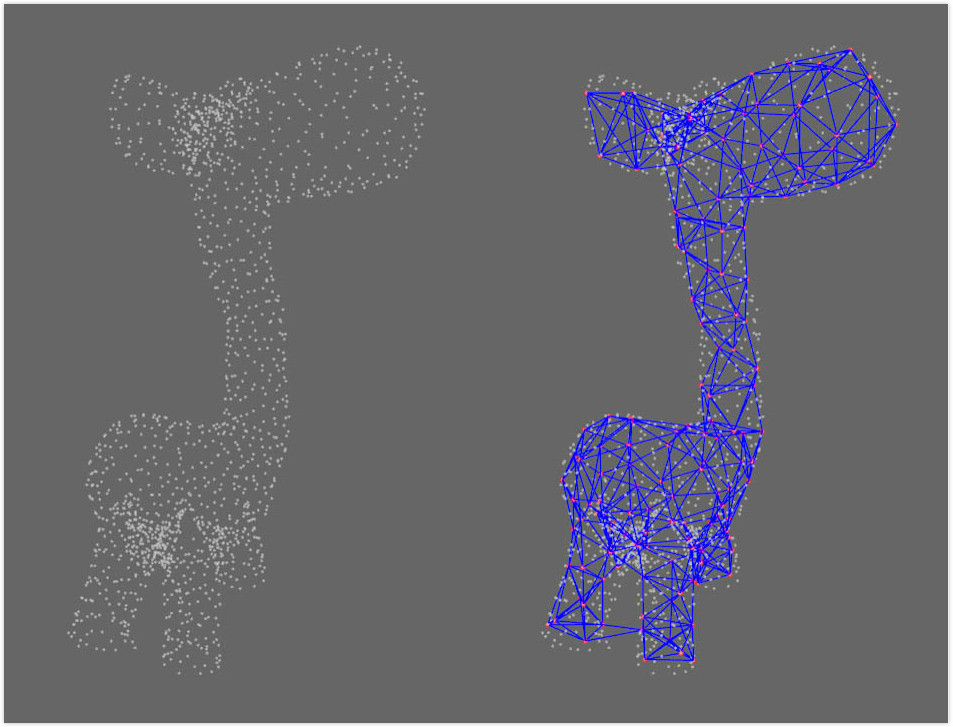
\includegraphics[width = \textwidth]{./Pictures/build_graph.jpg}
    \caption{构建形变图}
    \label{build_graph}
\end{figure}
\begin{algorithm}
    %\fangsong
    \caption{生成形变图边}
    \label{alg_gen_edges}
    \begin{algorithmic}[1]
        \Function {GenerateEdges}{$\bm{Node}$,$k_e$}
            \For{$\forall node_i \in \bm{Node}$}
                % find k-nearest nodes $node_j$ of $node_i$
                %  and build $edge_{ij}$ form $node_i$ to $$
                \For{all $k_e$ nearest nodes $node_j$ of $node_i$}
                    \State $edge_{ij} \gets$ build edge for $node_i$ to $node_j$
                    \State $\bm{Edge} \gets \bm{Edge} \bigcup \{edge_{ij}\}$
                \EndFor
            \EndFor
            \State \Return $\bm{Edge}$
        \EndFunction
    \end{algorithmic}
\end{algorithm} 

构建了形变节点和连接相邻节点的边,形变图本身的结构和性质以及确定,
但还需要确定形变图节点与模型顶点的对应关系,
即确定每个顶点的刚体变换由哪些顶点的刚体变换插值得到。
如同上一节中所说,本文采用k最近邻策略确定控制每个模型顶点的形变节点。
对于模型中的顶点$\bm{v}$,选取形变图中离它最近的$k_v$个形变节点,
作为该节点的控制节点。
在形变过程计算顶点$\bm{v}$发生的刚体变换由它所有的控制节点的刚体形变插值得到。
由于模型顶点和形变图节点的控制关系是通过未发生形变时的位置确定的,
这一关系在形变的过程中并不会改变。
所以控制关系只需要在确定了形变图结构后计算一次并记录下来。
算法\ref{alg_knn_nodes}描述了这一过程。
与生成边的步骤中一样,
k最近邻形变节点可以借助事先构建的KD Tree快速查找。
\begin{algorithm}
    %\fangsong
    \caption{生成形变图边}
    \label{alg_knn_nodes}
    \begin{algorithmic}[1]
        \Function{FindKnnNodesForVertex}{$\bm{Node}$,$\bm{V_{mesh}}$, $k_v$}
            \For{$\forall \bm{v} \in \bm{V_{mesh}}$}
                \State $\bm{Node_{knn}} \gets$ get $k_v$ nearest nodes of $\bm{v}$
                \State $\bm{GN}(\bm{v}) \gets \bm{Node_{knn}}$
            \EndFor
            \State \Return $\bm{GN}$
        \EndFunction
    \end{algorithmic}
\end{algorithm} 

% \begin{algorithm}
%     %\fangsong
%     \caption{形变图构建}
%     \label{alg_build_graph}
%     \begin{algorithmic}[1]
%         \Procedure{BuildGraph}{$\bm{V_{mesh}}$,$r_G$,$k_e$,$k_v$}
%             %\State build KD Tree with $\bm{V_{mesh}}$
%             \State $\bm{Node} \gets$ \Call{GenerateNodes}{$\bm{V_{mesh}}$,$r_G$}
%             %\State build KD Tree with $\bm{Node}$
%             \State $\bm{Edge} \gets$ \Call{GenerateEdges}{$\bm{Node}$,$k_e$}
%             \State $\bm{GN} \gets$ \Call{FindKnnNodesForVertex}{$\bm{Node}$,$\bm{V_{mesh}}$, $k_v$}
%         \EndProcedure
%         \Function{GenerateNodes}{$\bm{V_{mesh}}$,$r_G$}
%             %\State $KDTree \gets$ build KD-Tree with all vertices in $V_{mesh}$
%             \State $\bm{V_{uncovered}} = \bm{V_{mesh}}$
%             \While{$\bm{V_{uncovered}} \neq \varnothing $}
%                 \State $\bm{v_r} \gets$ randomly select a vertex in $V_{uncovered}$
%                 \State $node.\bm{vn} \gets \bm{v_r}$
%                 \State $\bm{Node} \gets \bm{Node} \bigcup \{node\}$
%                 \State $\bm{V_{uncovered}} \gets \bm{V_{uncovered}} - 
%                         \{\bm{v} \in \bm{V_{uncovered}} \quad | \quad 
%                         \|\bm{v} - \bm{v_r}\| \leq r_G\}$
%             \EndWhile
%             \State \Return $\bm{Node}$
%         \EndFunction
%         \Function {GenerateEdges}{$\bm{Node}$,$k_e$}
%             \For{$\forall node_i \in \bm{Node}$}
%                 % find k-nearest nodes $node_j$ of $node_i$
%                 %  and build $edge_{ij}$ form $node_i$ to $$
%                 \For{all $k_e$ nearest nodes $node_j$ of $node_i$}
%                     \State $edge_{ij} \gets$ build edge for $node_i$ to $node_j$
%                     \State $\bm{Edge} \gets \bm{Edge} \bigcup \{edge_{ij}\}$
%                 \EndFor
%             \EndFor
%             \State \Return $\bm{Edge}$
%         \EndFunction
%         \Function{FindKnnNodesForVertex}{$\bm{Node}$,$\bm{V_{mesh}}$, $k_v$}
%             \For{$\forall \bm{v} \in \bm{V_{mesh}}$}
%                 \State $\bm{Node_{knn}} \gets$ get $k_v$ nearest nodes of $\bm{v}$
%                 \State $\bm{GN}(\bm{v}) \gets \bm{Node_{knn}}$
%             \EndFor
%             \State \Return $\bm{GN}$
%         \EndFunction
%     \end{algorithmic}
% \end{algorithm} 
\section{形变参数优化}
在模型表面生成形变图之后,
就可以通过形变图中各节点的参数控制模型的形状。
本文将这些形变节点的参数成为模型的形变参数。
形变捕捉步骤就是通过优化形变参数,
使得模型的形状与深度相机捕捉的物体形状尽可能一致。
\subsection{形变优化流程}
在形变捕捉步骤中,本文的输入是深度视频。
对于视频的每一帧,
本文会优化模型的形变参数。
对于网格模型中的一个顶点$\bm{v_i}$,
它在每一帧的位置位置由两个变换决定。
第一个变换是整个模型在空间中发生的刚体变换$\bm{T_{rigid}}$,
这部分变换被为模型刚体变换;
第二个变换是根据形变图计算出的该节点的变换$G(\bm{v_i}=)Q2T(\hat{\bm{q_{v_i}}})$,
这部分变换被称为模型的非刚体变换。
形变后的模型中顶点的新位置为$\bm{v_i^{'}}=G(\bm{v_i})\bm{T_{rigid}}\bm{v_i}$。
本文需要计算的就是每一帧中的这两个变换。
图\ref{deformation_sampling}描述了形变捕捉的流程。
\begin{figure}
    \centering
    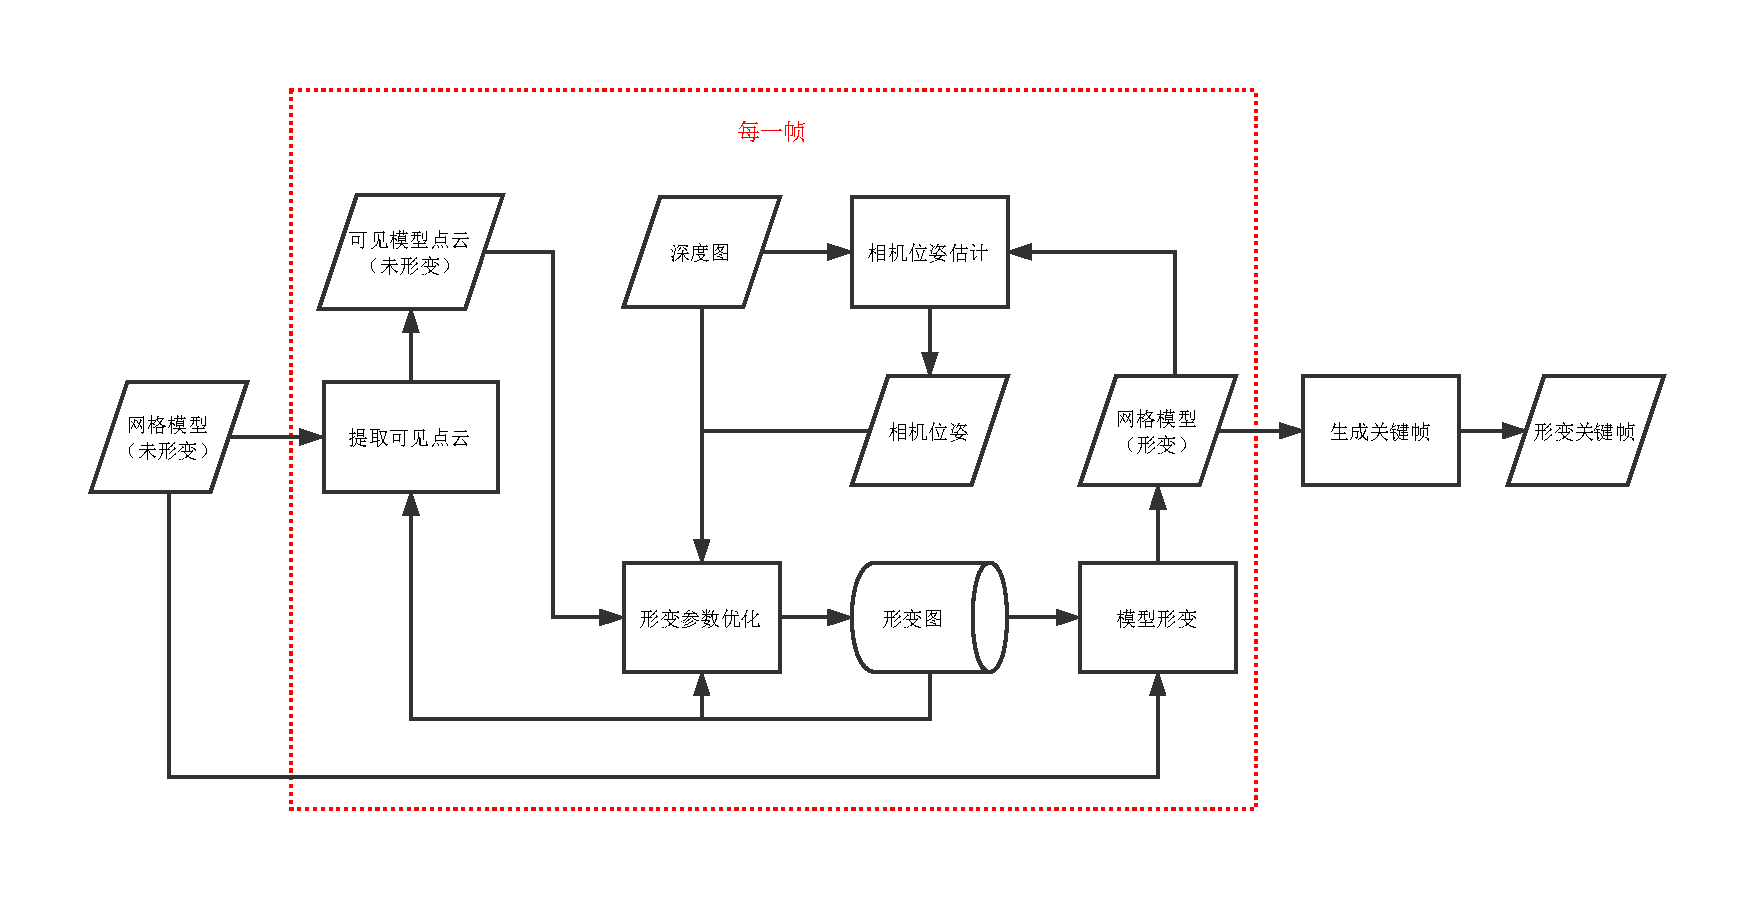
\includegraphics[width = \textwidth]{./Pictures/ds_pipeline_cropped.pdf}
    \caption{形变捕捉流程}
    \label{deformation_sampling}
\end{figure}
首先,本文将根据公式\ref{eq_d2v}将输入的深度图像转换为相应的三维点云。
在采集的深度视频中,操作者手部的深度信息也会被采集。
这些手部的深度信息对于形变捕捉来说是噪声,
本文会通过颜色过滤去除那些深度图像中可能是手部的区域。
由于在形变捕捉步骤中,仅有模型所在的区域(通过模型的透视投影获得)的深度信息会参与运算,
所以在这一阶段并不需要像确定初始位姿时通过深度过滤和最大连通域进一步分割属于物体的区域。
无论是计算模型的刚体变换还是模型的非刚体变换,
这个点云均被看做模型的参照。

然后,本文会计算当前帧点云相对于上一帧点云的相对刚体变换$\bm{T_{\epsilon }}$。
本文采用ICP算法估计刚体变换$\bm{T_{\epsilon }}$。
ICP算法的输入分别是当前帧的点云,和上一帧形变后的网格模型。 
将ICP计算得到的相对刚体变换叠加到上一帧的上一帧模型刚体变化上,
就能得到当前的模型刚体变换。
\begin{equation}
    \bm{T_{rigid}}=\bm{T_{\epsilon}}\bm{T_{rigid}^{pre}}
\end{equation}
非刚体部分的变换本质上是估计物体和相机的相对位置的变换,
所以图\ref{deformation_sampling}中将这一步骤称为相机位姿估计。

在计算了模型的刚体变换后,本文会优化模型的形变参数,
使得模型在形变后的形状尽量和深度图转换获得的点云接近。
这是一个参数为形变图各节点的双四元数值的最优化问题,
优化的能量函数为:
\begin{equation}
    E(\bm{Node},\bm{Edge},\bm{mesh},\bm{D})=DE(\bm{Node},\bm{mesh},\bm{D})+
    \lambda RE(\bm{Node},\bm{Edge})
\end{equation}
其中,$\bm{D}$为输入的深度图像,$\bm{mesh}$为网格模型;
$\bm{Node}$和$\bm{Edge}$分别为形变图的节点和边的集合;
$DE$为数据能量项,描述了形变后的模型和捕捉到的点云之间的误差;
$RE$为正则项,用来保证形变图的平滑性;
$\lambda$是正则项的权重系数,用来控制形变图中相邻节点间约束的强度;
该优化问题中,优化变量为$\bm{Node}$中各节点中双四元数的值,
关于数据项和正则项的具体形式,下面的章节会做详细的描述。

上述优化的结果将用于更新形变图,
从而改变形变后模型的形状。
如图\ref{deformation_sampling}中所示,
每一帧优化后得到的形变模型将用于估计下一帧的估算相机位姿的输入;
更新后形变图也将用于下一帧分析模型可见性以及数据对应关系的依据。

在形变捕捉的过程中,上述步骤不断重复,
每一帧都会得到一个与深度图像相对应的形变后的网格模型。
本文会从中挑选出一些模型用以构造形变关键帧。
图\ref{deformation_sampling_demo}显示了形变捕捉的结果,
左边的大图显示了将形变后的网格模型按照深度相机的相机的相机参数渲染到RGB图像上的结果;
右边的四张图分别是根据颜色过滤后的深度图生成的法向图、RGB图像、形变前的网格模型、
形变后的网格模型。

\begin{figure}
    \centering
    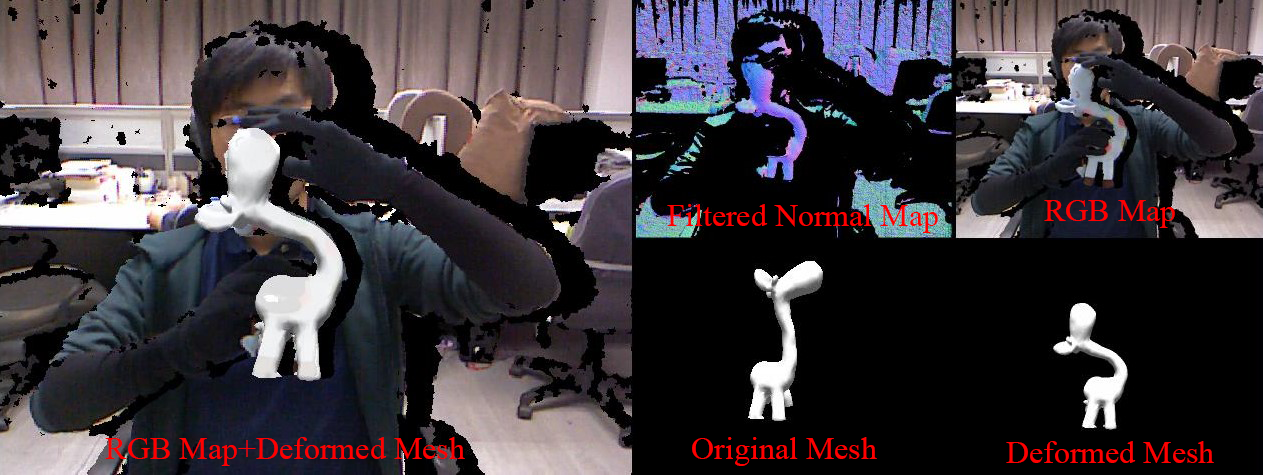
\includegraphics[width = \textwidth]{./Pictures/defSamp.png}
    \caption{形变捕捉结果}
    \label{deformation_sampling_demo}
\end{figure}
\subsection{数据能量项}
优化形变参数的目标是让形变后的模型形状和深度相机捕捉到的物体形状尽可能接近,
数据能量项就描述了形变后的模型和捕捉到点云之间的误差。

要对两组数据进行比较,首先要确认两组数据间的对应关系。
由于相机只能捕捉到物体朝向相机的那一面的信息,
所以模型中也只有形变后朝向相机的那一部分能有与之对应的深度信息。
这一部分即用深度相机的相机参数对形变后的模型进行三维渲染时被渲染出来的那部分模型,
本文称之为可见模型。
本文会预判模型表面各点在当前帧的可见性,提取出一组可见的点云作为形变图的输入。
对于每一帧,本文都构建了一个从像素坐标到形变模型上对应点在形变前的坐标和法向的映射。
即给定一个像素空间内的坐标$\bm{u}$,能够得到一个顶点坐标$\bm{vo_u}$和法向$\bm{no_u}$,
分别记录了形变模型中投影到像素位置$\bm{u}$处的三维点$\bm{vd_u}$在形变前的位置和法向。
本文会在每一帧计算出一张模型顶点图$\bm{VO}$和一张模型法向图$\bm{NO}$
其尺寸与深度图$\bm{D}$相同,
每个像素分别存储了该像素点对应的初始模型顶点$\bm{VO}(\bm{u})=\bm{vo_u}$
和初始法向$\bm{NO_u}(\bm{u})=\bm{no_u}$,这些点的信息构成了可见模型点云。
这两张图可通过栅格化渲染管线得到。
计算这两张图的过程
可看做渲染形变模型时分别用初始顶点坐标和初始法向作为模型顶点的颜色进行栅格化渲染。
其中的形变模型是根据上一帧更新后的形变图得到的。
此外,如上小结所述,本文还会从当前的深度图生成相应的顶点图$\bm{VD}$,
它的像素中存储了对应的点云顶点位置$\bm{VD}(\bm{u}) = \bm{vd_u}$,
其中$\bm{vd_u}=\bm{D}(\bm{u})\bm{K}^-1[\bm{u},1]$。
数据能量项的定义如下:
\begin{equation}
    DE(\bm{Node},\bm{mesh},\bm{D})=
    \sum \psi_{DE}(
        \hat{\bm{no}}_{\bm{u}}^T
        (
            \hat{\bm{vo}}_{\bm{u}}
            -
            \bm{vd_{\widetilde{\bm{u}}}}
        )
    )
\end{equation}
其中
\begin{align}
    &\hat{\bm{no}}_{\bm{u}}=G(\bm{vo_u})\bm{no_u}=G(\bm{VO}(\bm{u}))\bm{NO}(\bm{u})\\
    &\hat{\bm{vo}}_{\bm{u}}=G(\bm{vo_u})\bm{vo_u}=G(\bm{VO}(\bm{u}))\bm{VO}(\bm{u})
\end{align}
分别为可见模型点云根据形变图形变后的顶点坐标与法向量。
$\bm{vd_{\widetilde{\bm{u}}}}$为与其对应的深度图点云$\bm{VD}$中的顶点。
$\widetilde{\bm{u}}$为$\bm{vo_u}$以深度相机的相机参数经过透视投影得到的像素位置。
可以看出$DE$中的每一项是可见点云和深度点云中对应点的连线在模型表面法向上的投影,
即深度点云到中的点到模型表面的距离。
如同DynamicFusion中的数据项,本文采用Tukey惩罚函数提高优化模型的鲁棒性。
$\psi_{de}(f)$即为Tukey惩罚函数:
\begin{equation}
    \psi_{de}(f)= 
    \begin{cases}
        \frac{\epsilon_{de}^2}{6}(1-(1-(\frac{f}{\epsilon_{de}})^3))
        &\quad |f|\leq\epsilon_{de}\\

        \frac{\epsilon_{de}^2}{6}
        &\quad |f|>\epsilon_{de}
        
    \end{cases}
\end{equation}
\subsection{相邻节点约束}
如上一节所说,深度相机只能捕捉到物体朝向相机的那一面的信息。
本文将这一面称为正面,将采集不到的一面称为背面。
模型中只有正面的点才能找到对应的匹配点,
所以也只有位于正面的形变图节点会影响数据能量项的值。

如果优化模型的能量项中只有数据能量项,
优化过程中只有那些影响了数据能量项的节点会被更新,
得到不正确的优化结果。
所以需要在优化模型的能量函数中添加相邻节点间的约束,
使得正面节点的变换能够通过相邻节点间的约束传递到背面。
\begin{equation}
    RE(\bm{Node},\bm{Edge})=
    \sum_{i}^{n}
    \sum_{j \in \bm{Neig}(i)}
    \psi_{re}(
            Q2T(
                \hat{\bm{q_i}}
            )
            \bm{vn_i}
            -
            Q2T(
                \hat{\bm{q_j}}
            )
            \bm{vn_j}
        )
\end{equation}
其中$\bm{Neig}(i)={j \quad | \quad \exists edge_{ij} \in \bm{Edge}}$
包含了所有$node_i$的相邻节点的编号。
可以看出$RE$描述的相邻节点的变换的差别。
添加这一能量项的目的是让优化的结果中相邻节点的变换尽可能接近,
即让局部的变换尽可能的保持刚体变换(As Rigid As Possible),
该约束能够让形变的过程中保持模型的局部特征。
$\psi_{re}(\bm{v})$为Huber惩罚函数,是一个能保持不连续性的惩罚函数
\begin{equation}
    \psi_{re}(\bm{v}) = 
    \begin{cases}
        \frac{1}{2}\|\bm{v}\|^2
        &\quad \|v\| \leq \epsilon_{re}\\
        \epsilon_{re}(\|\bm{v}\|-\frac{\epsilon_{re}}{2})
        &\quad \|v\| > \epsilon_{re}
    \end{cases}
\end{equation}
\section{提取形变关键帧}
本文将用来构建形变子空间的形变模型称为形变关键帧,
这些形变关键帧通常为该物体较为典型的形变状态。
在形变捕捉步骤中,本文会计算每一帧模型的形变参数,
获得每一帧和深度图像相匹配的形变模型。
形变模型中每个顶点的位置由未形变模型的顶点位置在当前时刻的形变图变换得到。
本文会从这些形变模型中人为挑选一些具有代表性的形变模型,
作为用于构建形变子空间的形变关键帧。

但形变捕捉过程中的获得的形变模型并不能直接用于形变子空间的构建。
其一,形变捕捉是根据深度图像采集的形状优化模型的形变参数,
而深度图像仅包含物体朝向相机的那一面的形状信息,背向相机的那一面的形状是未知的。
背面的形状是通关相邻形变节点间的约束由正面传递过去的,可能并不准确。
其二,由于累计误差,各帧获得的形变模型在空间中并未对齐,
这会导致有此构建的形变子空间包含了冗余的变换信息。
本节就会描述解决上述问题的方法。
\subsection{多视角关键帧合成}
为了解决模型背面形变不准的问题,
本文给出了一种合成多个形变模型的方法。
对于同一形态的物体,操作者可以在不同视角下采集数据,
每个视角各自生成一个形变模型,
然后将这些模型合成为一个模型。

本文将一个视角下的形变模型称为子关键帧。
对于每一个子关键帧,本文将该模型中的顶点分为可见部分与不可见部分。
可见部分即模型中朝向相机的部分。
本文将包含第$k$个子关键帧中所有可见顶点的集合称为$\bm{V_{visible}^k}$。
对于第$k$子关键帧中的顶点$\bm{v_i^k}$,
其在相机坐标系中的位置为$\bm{T_{rigid}}\bm{v_i^k}$。
相机焦点在相机坐标系中位于原点$(0,0,0)$。
如果从原点$(0,0,0)$到$\bm{T_{rigid}}\bm{v_i^k}$的射线不与该子关键帧中任何不包含该顶点的面相交,
则顶点编号$\bm{v_i^k}$属于集合$\bm{V_{visible}^k}$。
本文定义了如下公式将$m$子关键帧的顶点合并:
\begin{equation}
    \widetilde{\bm{v}}_{\bm{i}} =
        \frac
            {\sum_{k=1}^{m} w(\bm{v_i^k})\bm{v_i^k}}
            {\sum_{k=1}^{m}w(\bm{v_i^k)}}
\end{equation}
其中
\begin{equation}
    w(\bm{v_i^k})=
    \begin{cases}
        w_v
        &\bm{v_i^k} \in \bm{V_{visible}^k}\\
        1
        &\bm{v_i^k} \notin \bm{V_{visible}^k}\\
    \end{cases}
\end{equation}
$w_v>1$为可见顶点的权重,本文的使用中设为2。
可以看出合成的方法为对各子关键帧的顶点加权平均,
每个子关键帧的可见顶点拥有更大的权重。
% \begin{equation}
%     \bm{ID_{v}} = \{ i \quad | \quad \bm{v_i} \in \bm{V_{mesh}}\ and\  
%     \nexists \bm{f} \in \bm{F_{mesh}} \quad the\ ray\ from (0,0,0)\ 
%     to\ G(\bm{v_i})\bm{T_{rigid}}\bm{v_i}\ intersect\ \bm{f}\}
% \end{equation}
% \begin{algorithm}
%     %\fangsong
%     \caption{获取可见顶点}
%     \label{alg_get_visible}
%     \begin{algorithmic}[1]
       
%         \Procedure{GetVisibleVertexes}{$\bm{mesh}$, $\bm{Node}$,$\bm{T_{rigid}}$,$\bm{K}$}
%              \State $\bm{mesh_{c}} \gets$ deform $\bm{mesh}$ with $\bm{Node}$ and transform it with $\bm{T_{rigid}}$
%              \For{$\forall \bm{arg}$}
%         \EndProcedure
%     \end{algorithmic}
% \end{algorithm}
\subsection{关键帧对齐}
从捕捉到的形变状态中提取关键帧时,
本文会去处模型的整体刚体变换$\bm{T_{rigid}}$,
提取的模型仅更具形变图更新顶点位置。
但形变图本质上是控制每个顶点在空间的刚体变换,
其中可以包含整个模型的刚体变换,如图\ref{before_after_align}(左)所示。
\begin{figure}
    \centering
    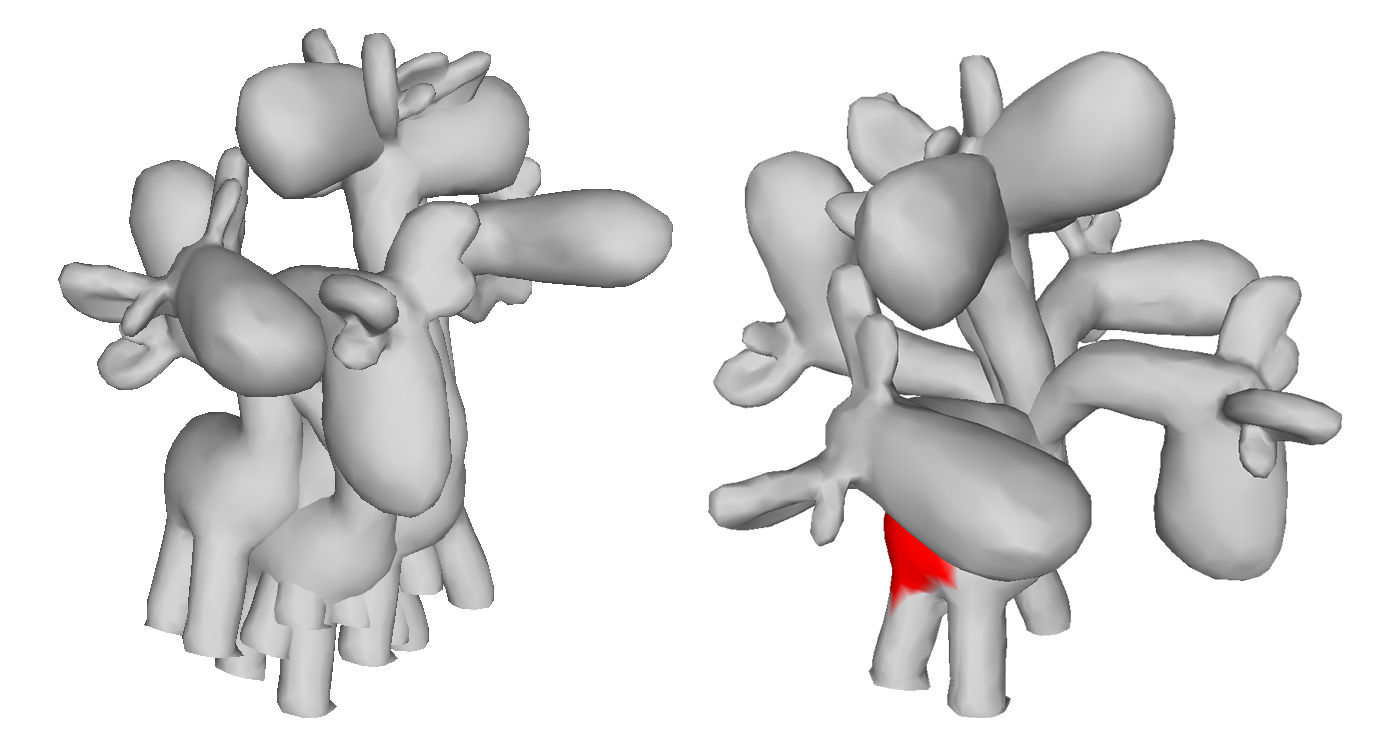
\includegraphics[width = \textwidth]{./Pictures/before_after_align.png}
    \caption{对齐前的关键帧}
    \label{before_after_align}
\end{figure}

在每一帧的形变捕捉计算中,
每次估计的$\bm{T_{rigid}}$都会存在误差。
如同上文所述,
每个顶点的空间变换由模型整体变换$\bm{T_{rigid}}$和由形变图描述的顶点变换$G(\bm{v})$两部分组成。
$\bm{T_{rigid}}$部分微小的偏移量可能会在形变参数优化时由$G(\bm{v})$部分补足。
每一帧的误差可能很小,但这些误差会逐帧积累,
导致提取出的关键帧存在整体偏移。
在构建形变子空间时从关键帧中提取的特征向量描述的是关键帧关于初始模型的相对形变。
这些整体偏移的平移部分对特征向量没有影响,
但是其旋转分量会导致从关键帧中提取的特征向量包含冗余的旋转信息。
所以本文需要消除这些偏移。
\begin{figure}
    \centering
    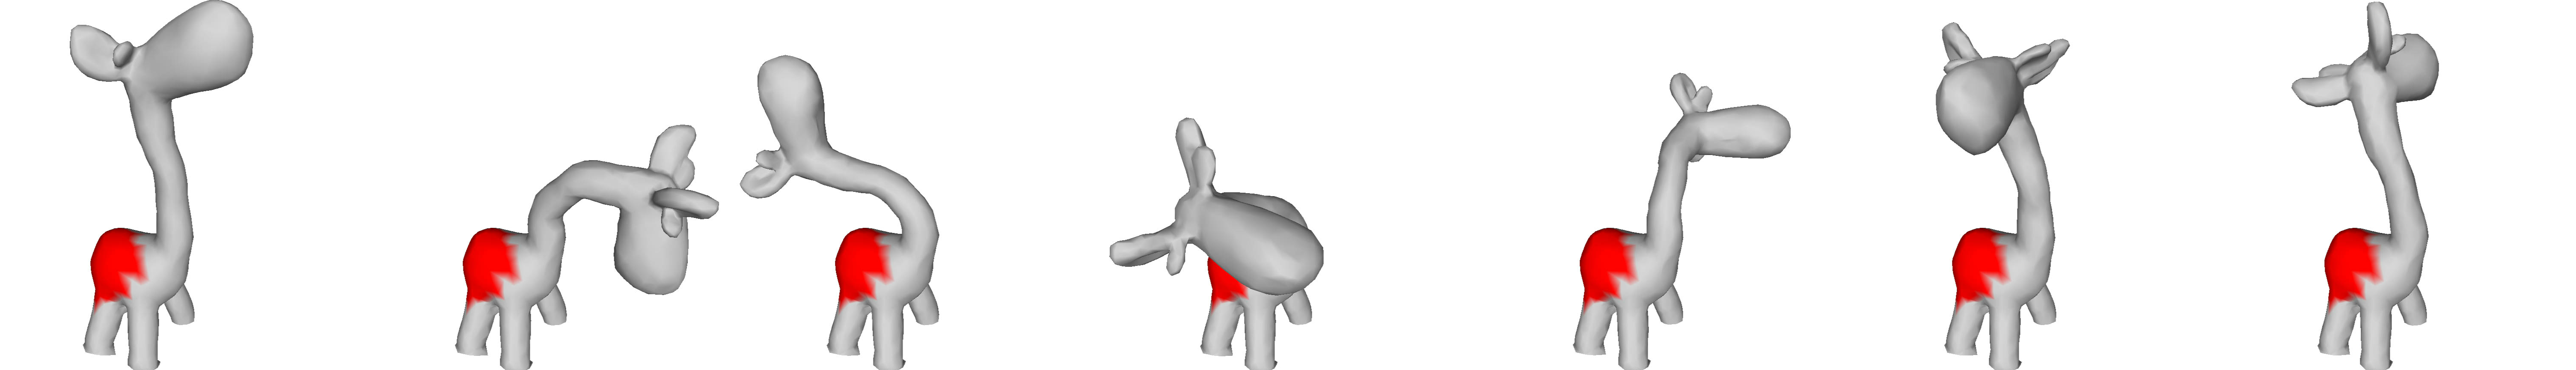
\includegraphics[width = \textwidth]{./Pictures/align_area.png}
    \caption{模型中用于对齐的区域}
    \label{align_area}
\end{figure}
本文采用的策略是选取模型中的一部分顶点,
各关键帧均用这部分顶点用ICP算法向初始模型对齐。
这个用于区域需要在形变捕捉的过程中是未发生形变的,
这样能提取出关键帧够尽可能保留模型的形变信息。
本文用初始位姿估计时被手覆盖的区域作为用于对齐的的区域。
图\ref{align_area}分别为初始模型和6个关键帧,
模型中红色的部分为用于对齐区域。
图\ref{before_after_align}(右)为对齐后的初始模型和形变关键帧。
% \begin{figure}[h]
%     \centering
%     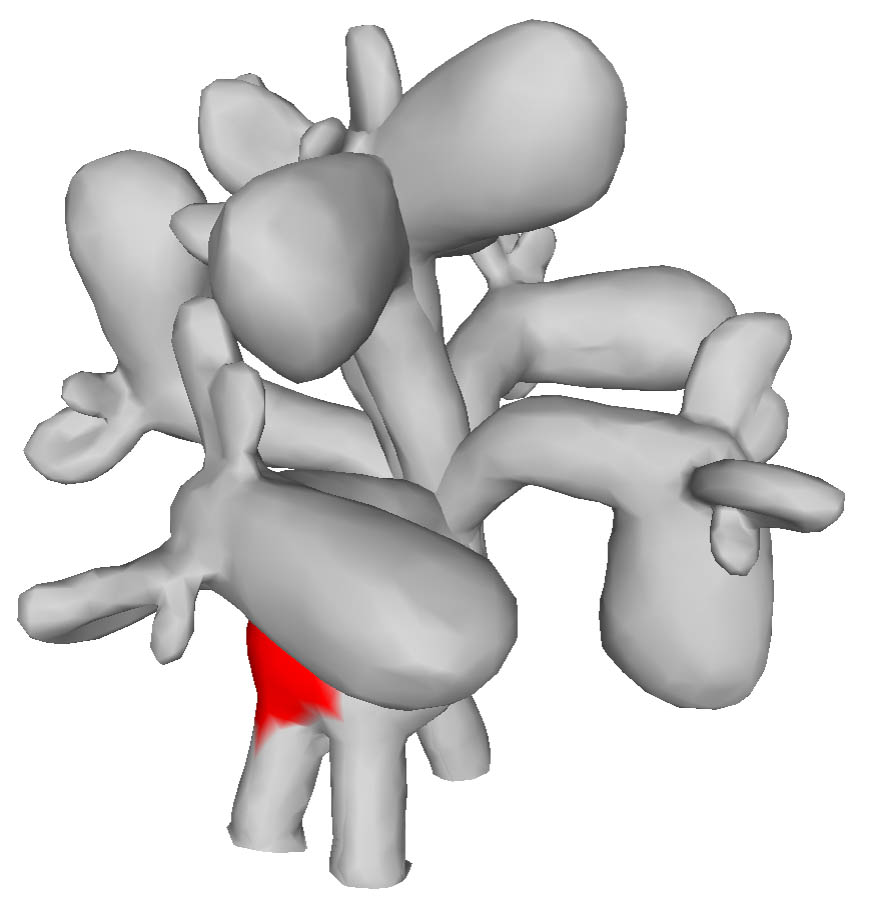
\includegraphics[width = 0.45\textwidth]{./Pictures/after_align.jpg}
%     \caption{对齐后的关键帧}
%     \label{after_align}
% \end{figure}
\section{本章小结}
本章描述了基于深度视频捕捉模型形变并生成形变关键帧的过程。
首先,本章介绍了双四元数的定义和性质,给出了形变框架的数学基础;
然后本章介绍了本文的形变框架,
描述了基于双四元数的形变图的定义、结构及其构造过程;
之后本章介绍了形变捕捉的流程,给出了形变参数优化问题的定义,
并消息介绍了能量函数的含义;
最后本章介绍从捕捉到的形变模型中提取关键帧的过程,
描述了多角度关键帧合成和关键帧对齐的方法。


\chapter{基于形变梯度的形变子空间构建}
本章将描述构建形变子空间的方法,
并给出了一个基于形变子空间的修改模型形状的算法。
形变子空间构建的输入是一个参考模型和一组形变关键帧。
本文会从每一个形变关键帧中提取出一个特征向量,
作为形变子空间的基向量。
这个特征向量描述的形变关键帧相对于参考模型的相对形变,
由模型中各三角面片的形变梯度组成。
由所有特征向量张成的空间被称为模型的特征空间,
空间中向量均可由基向量非线性插值得到。
特征空间中的向量对应的形变模型组成了模型的形变子空间。
本文还给出了一个基于形变子空间修改模型形状的算法,
可以让用户通过拖动控制点得到符合物体形变特征模型形状。
\section{基于形变梯度的形变子空间}
本文基于网格模型中面片的形变梯度从形变关键帧中提取特征向量,
这些特征向量张成的空间被称作该模型的特征空间。
本节将详细介绍形变梯度的概念,描述特征向量和网格模型互相转换的方法,
以及特征向量在非线性空间进行插值的方法。
\subsection{形变梯度}
形变梯度是一组三维点在三维空间中发生的仿射变换的雅可比矩阵。
参考模型即未发生形变的模型,在本文中即第三章中重建的三维模型。
本文描述的形变梯度是在三角面片上定义的。
Sumner的相关工作\cite{sumner2004deformation}曾经用形变梯度进行模型间的形变转移。
本文中形变子空间构建的方法借鉴了Sumner的MeshIK\cite{sumner2005mesh}。

将三角面片发生的仿射变换记为$\Phi$:
\begin{equation}
    \label{eq_at}
    \Phi(\bm{v})=\bm{T}\bm{v}+\bm{t}
\end{equation}
其中$3 \times 3$矩阵$\bm{T}$包含了旋转变换、缩放变换和斜切变换,
三维向量$\bm{t}$包含了三维空间中的平移变换;
$\bm{v}$为三维空间中的点。
可以看出$\Phi$关于三维向量$\bm{v}$的梯度为变换矩阵$\bm{T}$。
\begin{figure}
    \centering
    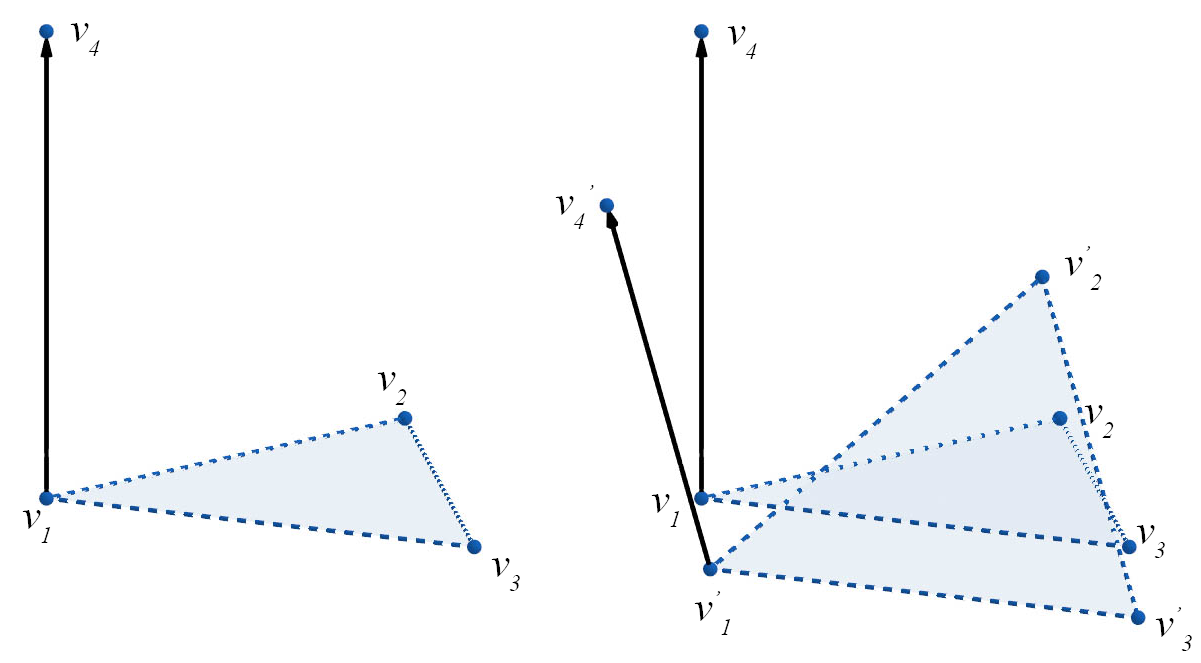
\includegraphics[width = 0.8\textwidth]{./Pictures/DefGra.png}
    \caption{三角面片的顶点四元组}
    \label{deformation_gradient}
\end{figure}

三角面片包含三个不共线的点$\bm{v_1}$、$\bm{v_2}$、$\bm{v_3}$,
但这三个点不足以定义三维空间中的放射变换,
因为这一组点无法定义面片法线方向上的上缩放变换。
所以计算形变梯度时需要加入第四个点$\bm{v_4}$,
组成该面片的顶点四元组。
\begin{equation}
    \bm{v_4}=\bm{v_1}
    +
    \frac
        {(\bm{v_2}-\bm{v_1})\times(\bm{v_3}-\bm{v_1})}
        {\sqrt{|(\bm{v_2}-\bm{v_1})\times(\bm{v_3}-\bm{v_1})|}}
\end{equation}
可以看出$\bm{v_{14}}=\bm{v_4}-\bm{v_1}$是垂直于面片的向量。
$\bm{v_{14}}$的方向通过$\bm{v_{12}}=\bm{v_2}-\bm{v_1}$和
$\bm{v_{13}}=\bm{v_3}-\bm{v_1}$的外积计算得到;
$\bm{v_{14}}$的长度为$\sqrt{|(\bm{v_2}-\bm{v_1})\times(\bm{v_3}-\bm{v_1})|}$,
这保证当面片发生仿射变换时,
$\bm{v_{14}}$会与$\bm{v_{12}}$和$\bm{v_{13}}$等比缩放。
仿射变换后的四个点分别为$\bm{v_1^{'}}$、$\bm{v_2^{'}}$、$\bm{v_3^{'}}$、$\bm{v_4^{'}}$。
若只考虑这四点的相对位置,则平移向量$\bm{t}$为0。
分别将$\bm{v_{41}}$、$\bm{v_{42}}$、$\bm{v_{43}}$代入公式\ref{eq_at},
得到
\begin{equation}
    \begin{aligned}
        &\bm{v_1^{'}}-\bm{v_4^{'}}=\bm{T}(\bm{v_1}-\bm{v_4})\\
        &\bm{v_2^{'}}-\bm{v_4^{'}}=\bm{T}(\bm{v_2}-\bm{v_4})\\
        &\bm{v_3^{'}}-\bm{v_4^{'}}=\bm{T}(\bm{v_3}-\bm{v_4})
    \end{aligned}
\end{equation}
以上方程组可改写成矩阵形式$\bm{V^{'}}=\bm{T}\bm{V}$,
其中
\begin{eqnarray}
     \bm{V}    &=&[\bm{v_1}-\bm{v_4},\bm{v_2}-\bm{v_4},\bm{v_3}-\bm{v_4}] \nonumber \\
     \bm{V^{'}}&=&[\bm{v_1^{'}}-\bm{v_4^{'}},\bm{v_2^{'}}-\bm{v_4^{'}},\bm{v_3^{'}}-\bm{v_4^{'}}]
\end{eqnarray}
$\bm{V}$与$\bm{V^{'}}$均为$3 \times 3$的矩阵,每一列分别为三个相对向量。
由此可以得到三角面片的形变梯度$\bm{T}$
\begin{eqnarray}
    \label{eq_def_grad}
    \bm{T}
    &= &\bm{V^{'}}\bm{V^{-1}} \nonumber \\
    &= &[\bm{v_1^{'}}-\bm{v_4^{'}},\bm{v_2^{'}}-\bm{v_4^{'}},\bm{v_3^{'}}-\bm{v_4^{'}}]\cdot \nonumber \\
    &\ &[\bm{v_1}-\bm{v_4},\bm{v_2}-\bm{v_4},\bm{v_3}-\bm{v_4}]^{-1}
\end{eqnarray}
\subsection{基于形变梯度的特征向量}\label{sec_feature}
本文会从每一个形变关键帧中提取一个基于面片形变梯度的特征向量。
给定一个参考模型$\bm{P}$和一个形变关键帧$\bm{K}$,
它们都包含$n$个顶点和$m$个面片。
对于$\bm{K}$中的每一个面片,都可以计算出相应的形变梯度$\bm{T}$。
由公式\ref{eq_def_grad}可知,当参考模型中的顶点位置确定,即为常数时,
形变梯度$\bm{T}$中各元素的值均为形变模型(形变关键帧)中相应顶点坐标元素的线性组合。
所以可用如下矩阵乘法计算模型的特征向量:
\begin{equation}
    \label{eq_mat_get_f}
    \bm{f}=\bm{G}\bm{x}
\end{equation}
其中向量$\bm{x}=(x_1,...,x_{n+m},y_1,...,y_{n+m},z_1,...,z_{n+m}) \in \mathbb{R}^{3(n+m)}$
是是$n+m$个三维点的坐标值堆叠成长向量,
其中$n$个点为模型中的顶点,$m$个点为$m$个面片的第四点。
线性算子$\bm{G}$的元素的值仅由参考模型中顶点的位置决定,
它用于构造特征向量$\bm{f}\in\mathbb{R}^{9m}$。
特征向量$\bm{f}$由$m$个面片的形变梯度$\bm{T}$中的元素的值堆叠而成。
矩阵乘法$\bm{Gx}$根据公式\ref{eq_def_grad}计算了每个面片的形变梯度$\bm{T}$,
并将这$m$个$3 \times 3$矩阵中的元素堆叠到长向量$\bm{x}$中的元素的值堆叠而成。

线性算子$\bm{G}$为$9m\times 3(n+m)$的矩阵。
由公式\ref{eq_def_grad}可知,
每个顶点只会影响包含它的面片的形变梯度,
所以矩阵$\bm{G}$是一个稀疏矩阵。
且每一个顶点在不同维度的值在运算中具有相同的线性组合,
所以矩阵$\bm{G}$拥有如下对角分块的结构
\begin{equation}
    \bm{G}=
    \begin{bmatrix}
        \bm{G_d} &        & \\ 
         &       \bm{G_d} & \\ 
         &       &        \bm{G_d}
    \end{bmatrix}
\end{equation}
每个矩阵块$\bm{G_d}$是一个$3m \times (n+m)$的稀疏矩阵,
每一行仅有四个非零元素,
分别对应利用公式\ref{eq_def_grad}计算相应形变梯度时需要的四个顶点。
求解公式\ref{eq_mat_get_f}中的方程就可以从特征向量映射回顶点坐标。
但是由于特征向量与模型在空间中平移无关,
所以直接求解公式\ref{eq_mat_get_f}$\bm{x}$会有无穷多个解。
要求解$\bm{x}$需要确定或约束至少一个顶点的位置。
约束顶点的方法将在网格修改模型的章节中介绍。
\subsection{特征向量的非线性插值}
本文将从每个形变关键帧中提取出特征向量称为基向量,
将基向量张成的向量空间称为模型的特征空间,
特征空间中的向量对应的形变模型是本文认为合理的形变模型。
特征空间中的向量均可由基向量插值得到。
对于$k$个基向量,给定$k$维权重向量$\bm{w}$,
可得到插值后的特征向量
\begin{equation}
    \bm{f_w}=\bm{Intp}(\bm{w})
\end{equation}
其中$\bm{Intp}$为插值函数。

线性插值是最为常见的向量插值方法,
但并不适用于本文中特征向量的插值。
由于本文中特征向量是表示模型姿态的变换矩阵$\bm{T}$的线性变换,
所以对特征向量线性插值等价于对模型的姿态线性插值。
当变换矩阵$\bm{T}$中包含旋转时,
插值后的模型姿态会显得不自然。
这种姿态在旋转程度较大时尤为明显,
如图\ref{linear_vs_unlinear}(三)所示。
在本文的应用场景中,
只有当选取形变关键帧密集采样,
使得相近的关键帧中面片间仅有微小的旋转时,
线性插值才适用于特征向量的插值。
但这样的密集采样并不现实,
也使得形变子空间的构建失去了意义。
为了解决插值结果不自然的问题,
本文需要一种能够将旋转分量更自然的插值的方法将基向量张成特征空间。
本文采用的是一种基于极分解(polar decomposition)\cite{shoemake1992matrix}
和矩阵指数映射( matrix exponential map)\cite{murray2017mathematical}
\cite{trove.nla.gov.au/work/222715717}
的非线性插值方法。
图\ref{linear_vs_unlinear}中前两张图为两个形变关键帧,
用$1:1$的权重对二者的特征向量插值,
后两张图分别为线性插值和非线性插值的结果。
模型的特征空间就是由基向量通过这种插值方法张成的。
\begin{figure}
    \centering
    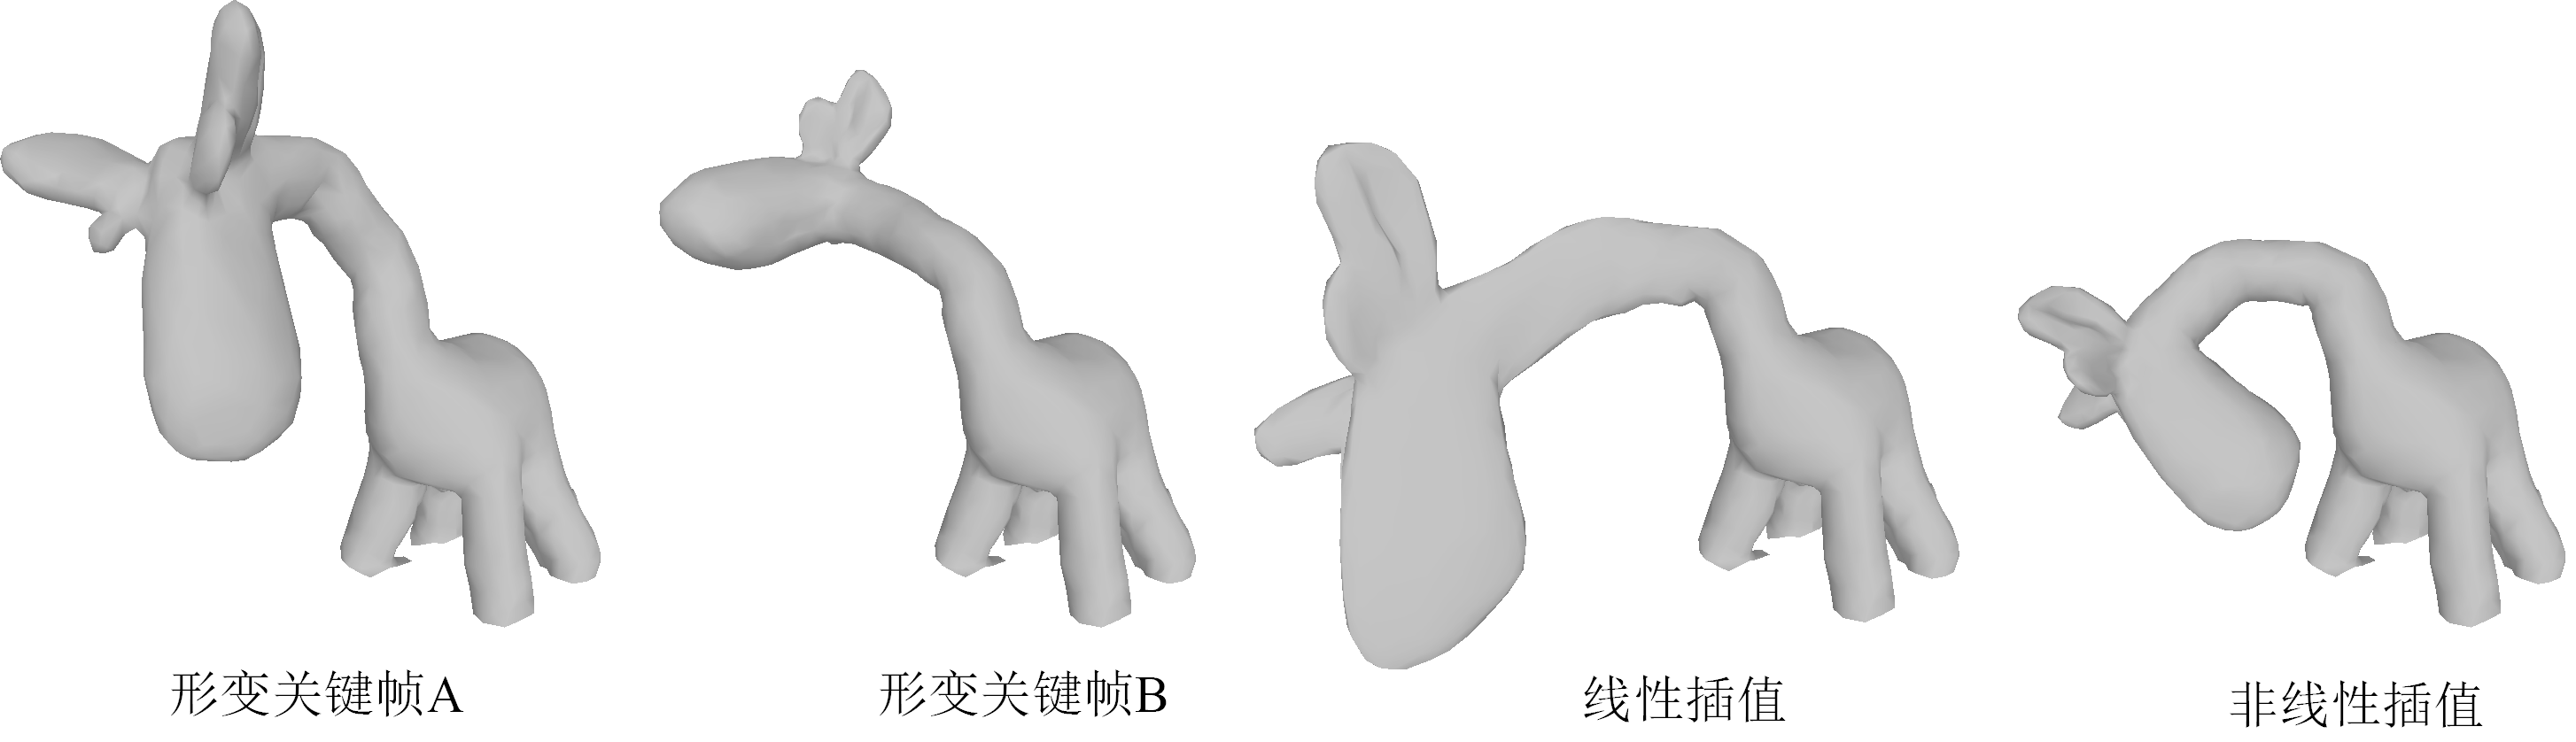
\includegraphics[width = \textwidth]{./Pictures/linear_vs_unlinear.png}
    \caption{特征的向量的插值方法}
    \label{linear_vs_unlinear}
\end{figure}

首先,用极分解将第$i$个形变关键帧中的第$j$个面片的形变梯度$\bm{T_{ij}}$
分解为旋转和缩放/切边两个部分:
\begin{equation}
    \bm{T_{ij}}=\bm{R_{ij}S_{ij}}
\end{equation}
这两部分会采用不同的插值策略。
其中缩放/切变部分$\bm{S_{ij}}$可直接使用线性插值,
而旋转部分$\bm{R_{ij}}$则需要做特殊处理。

本文在旋转分量的插值中运用了矩阵的指数映射和对数映射。
本节将简要介绍矩阵指数映射和对数映射的概念,
想了解更多细节和证明可查阅相关资料\cite{murray2017mathematical}
\cite{trove.nla.gov.au/work/222715717}。
这两种映射能够提供空间旋转在$\bm{SO}(3)$和$\mathfrak{so}(3)$间的转换。
其中$\bm{SO}(3)$为一个李群,称为三维旋转群,
是特殊正交群$\bm{SO}(n)$在$n=3$时的特例,
它包含了所有三维旋转矩阵。
$\mathfrak{so}(3)$为三维旋转群$\bm{SO}(3)$对应的李代数。
可以看做一组$3 \times 3$的反对称矩阵,
这些矩阵可有一个向量生成,
这个向量是三维正交群中的旋转矩阵对应旋转向量,
它们的对应关系可由罗德里格斯公式表明。
所以$\mathfrak{so}(3)$也可以看做是三维旋转向量组成的空间。
指数映射可以将$\bm{SO}(3)$中的旋转矩阵映射到$\mathfrak{so}(3)$,
对数映射为指数映射的逆映射。
在本文采用的插值方法中,
会利用指数映射将旋转矩阵从$\bm{SO}(3)$映射到$\mathfrak{so}(3)$,
在$\mathfrak{so}(3)$中做线性插值,然后将插值的结果用对数映射映射回
$\bm{SO}(3)$。
模型中第$j$个面片的形变梯度$\bm{T_j}$的非线性插值可由如下公式描述:
\begin{equation}
    \label{eq_unlinear}
    \bm{T_j}(\bm{w})
    =
        exp(\sum_{i=1}^{k}w_i\log (\bm{R_{ij}}))
        \cdot
        \sum_{i=1}^{k}w_i\bm{S_{ij}}
\end{equation}
其中$exp$和$log$分别为指数映射和对数映射,$w_i$为第$i$个基向量的权重。
特征向量中各面片的形变梯度均使用公式\ref{eq_unlinear}进行非线性插值,
即为特征向量的插值函数$\bm{Intp}(\bm{w})$。
\section{基于形变子空间的网格模型形状修改}
本节交描述一个基于形变子空间的模型修改方法。
用户可通过拖动控制点实现对模型形状的修改。
\subsection{形状优化模型}
如章节\ref{sec_feature}所述,
由于特征向量与模型的平移无关,
所以需要多模型中至少一个顶点的位置进行约束,
才能得到与指定特征向量对应的形变模型。
这可以用如下优化问题表示:
\begin{eqnarray}
    \bm{x}&=&arg\ \min_{\bm{x}} (E_f(\bm{x}) + E_c(\bm{x})) \nonumber \\
          &=&arg\ \min_{\bm{x}} (\|\bm{Gx}-\bm{f}\| + \lambda_c  \sum_{i=1}^{l}\|\bm{v_i}-\bm{vc_i}\|)
\end{eqnarray}
其中$E_f$为特征约束,可由公式\ref{eq_def_grad}得到,
将模型约束在形变空间内;
$E_c$为控制点约束,$\bm{vc_i}$为固定点的位置。
优化结果即为指定了固定点后特征向量$\bm{f}$对应的形变模型的顶点位置。
$E_c(\bm{x})$可改写为与$E_f$类似的矩阵形式:
\begin{eqnarray}
    E_c(\bm{x})&=&\|\bm{
        \bm{M_c}x}
        -
        \bm{f_c}\| \nonumber \\
    \bm{M_c}&=&
    \begin{bmatrix}
        \bm{G_c} &        & \\ 
         &       \bm{G_c} & \\ 
         &       &        \bm{G_c}
    \end{bmatrix}
\end{eqnarray}

当有$l$个固定点时,$\bm{G_c}$为$l \times (n+m)$的矩阵,
每行只有与固定点$\bm{v_i}$对应的一列非零,
值为权重$\lambda$。
$\bm{f_c}$为$3l$维的向量,
对应$3l$个固定点的坐标,
值为对应固定点坐标与固定点权重$\lambda$的乘积。
因为$E_f$与$E_c$有如此相近的形式,
可以将二者合并为一个能量。
有此可以得到新的优化问题:
\begin{equation}
    \label{eq_feature2mesh}
    \bm{x}=arg\ \min_{\bm{x}} \| \bm{\widetilde{G}x}-(\widetilde{\bm{f}}+\bm{c}) \|
\end{equation}
其中$\bm{\widetilde{G}}$为扩展后的$\bm{G}$,$\widetilde{f}$为扩展后的$\bm{f}$。
\begin{eqnarray}
    \bm{\widetilde{G}}&=&
    \begin{bmatrix}
        \bm{\widetilde{G_d}} &        & \\ 
         &       \bm{\widetilde{G_d}} & \\ 
         &       &                  \bm{\widetilde{G_d}}
    \end{bmatrix}\\
    \bm{\widetilde{G_d}}&=&
    \begin{bmatrix}
        \bm{G_d} \\ 
        \bm{G_c}
    \end{bmatrix}
\end{eqnarray}

若将公式\ref{eq_feature2mesh}中的$\bm{f}$替换为$\bm{f_w}=\bm{Intp}(\bm{w})$,
并将插值权重$\bm{w}$也作为优化变量,
以用户指定的控制点作为静止点,
就能得到修改模型形状的优化问题:
\begin{equation}
    \bm{x}=arg\ \min_{\bm{x},\bm{w}}
    \|
        \bm{\widetilde{G}x}
        -
        (\bm{Intp}(\widetilde{\bm{f}})+\bm{c}) 
    \|
\end{equation}
\section{本章小结}

 \chapter{结果分析}
 本文的实验均在安装了Windows 10专业版的台式机上完成,
 实验平台环境如表\ref{tab_pc}所示。
 用于采集数据的扫描设备参数如表\ref{tab_kinect}。
 本章的实验主要在三个样例上进行,
 这三个样例分别为giraffe、pillow和tube。
 这三个样例在现实中的样子和重建后模型如图\ref{static_model}所示。
 本章将展示更多本文的实验结果。
 章节\ref{sec_pose_est_res}将展示在不同的物体位姿下位姿估计算法的结果;
 章节\ref{sec_keyframe_res}将展示捕捉形变并提取关键帧的结果;
 章节\ref{sec_subspace_res}将展示形变子空间的相关结果。
\begin{table}[htp]
    \zihao{5}
    \caption{实验平台参数}
    \label{tab_pc} 
    \centering
    \begin{tabular}[t]{|l|l|c|}
        \hline
        \multirow{3}*   {硬件}  &    CPU        &   Intel® Core™ i5-4430 主频3.00GHz,四核四线程\\
        \cline{2-3}
                                &    GPU         &   NVIDIA GeForce GTX 760,显存4GB\\
        \cline{2-3}
                                &    内存        &   16GB\\
        \hline
        \multirow{2}*   {软件}  &    CUDA        &   CUDA 8.0\\
        \cline{2-3}
                                &    Kinect SDK  &   Kinect SDK 1.8\\
        \hline
    \end{tabular}
\end{table}
\begin{table}[htp]
    \zihao{5}
    \caption{扫描设备参数}
    \label{tab_kinect}
    \centering
    \begin{tabular}[t]{|l|c|}
        \hline
        扫描设备        &   Kinect for Xbox 360\\
        \hline
        RGB图像         &   分辨率$640 \times 480$,深度32位\\
        \hline
        深度图像        &   分辨率$640 \times 480$,深度16位\\
        \hline
        传感深度范围    &   1.2m-3.5m\\
        \hline
        % 最大FPS        &    30\\
        % \hline
    \end{tabular}
\end{table}
 \section{初始位姿估计结果}\label{sec_pose_est_res} 
 图\ref{align_result}展示了各样例的对齐结果。
 其中前两列为giraffe在两种不同位姿下的估计结果,
 第三列为pillow的估计结果,
 第四列为tube的估计结果。
 图中每一列为每一种位姿下位姿估计算法的结果;
 第一行为手部点云分割的结果,
 蓝色的像素为分割出的手部点云;
 第二行为物体点云分割的结果,
 红色的像素为分割出的物体点云;
 第三行为根据估计出的位姿将模型渲染到RGB图像的结果;
 第四行为直接将模型平移到物体点云包围盒中心后的结果;
 第五行为模型和物体点云对齐后的得结果模型以估计出的位姿变换。
 从图中可以看出,
 在各种位姿下,
 本文的算法都能准确的分割出点云并将其与模型对齐,
 从而估计出物体的位姿。
 最后的对齐结果中,
 调整位姿后的模型和根据深度图像生成的点云间仍然存在一定的偏移。
 但这样的对齐效果足够作为ICP算法的初值,
 用ICP算法做局部对齐消除偏移。
 在形变捕捉的过程中,
 每一帧都会用ICP算法估计物体的刚体变换,
 所以模型初始位姿中这些偏移不会对后续的算造成影响。
 \begin{figure}
    \centering
    \includegraphics[width = \textwidth]{./Pictures/align_result_muti_model.png}
    \caption{不同位姿下的位姿估计结果}
    \label{align_result}
\end{figure}
\begin{table}
    \zihao{5}
    \caption{物体点云分割数据}
    \label{tab_sample_data} 
    \centering
    \begin{tabular}[t]{|l|c|c|c|}
        \hline
        样例       &   顶点数   &   面片数   &  物体点云顶点数\\
        \hline
        giraffe     &   1551    &   3000    &   10189       \\
        \hline
        pillow      &   3008    &   6000    &   16090       \\
        \hline
        tube        &   5019    &   10000   &   11653       \\
        \hline
    \end{tabular}
\end{table}

表\ref{tab_sample_data}给出了各样例的基本属于以及初始位姿估计时分割出的物体点云的顶点数;
表\ref{tab_est_pose_time}为各样例在初始位姿估计各阶段的耗时。
表\ref{tab_est_pose_time}中将颜色过滤单独划出,
并不算在手部分割中,
是因为该步骤是在讲RGB图向深度图映射时在GPU上实现的,
这样只需要向GPU传输一次颜色数据。
物体点云分割耗时指的是获取手部点云后,
根据手部点云后根据手部位置寻找物体点云的耗时。
从表\ref{tab_est_pose_time}中可以看出,
用于点云分割的三个步骤耗时很小,
最耗时的是点云对齐。
点云对齐的耗时也与模型的大小无关,
因为对齐前会对物体点云和网格模型中的顶点均匀采样。
本文用于对齐的样本大小与分割出的物体点云中顶点的个数成正比,
所以点云对齐的耗时和物体点云的大小正相关。
\begin{table}
    \zihao{5}
    \caption{位姿估计耗时}
    \label{tab_est_pose_time} 
    \centering
    \begin{tabular}[t]{|l|c|c|c|c|c|}
        \hline
        样例        &   颜色过滤耗时   & 手部分割耗时    &   物体点分割耗时    & 点云对齐耗时    &   总耗时\\
        \hline
        giraffe    &    0.0376s       &  0.0087s       &    0.0336s         &   0.3973s     &   0.4773s\\
        \hline
        pillow     &    0.035s        &  0.0067s       &    0.0302s         &   0.7707s     &   0.8427s\\
        \hline
        tube       &    0.0309s       &  0.0109s       &    0.0317s         &   0.437s      &   0.5005s\\             
        \hline
    \end{tabular}
\end{table}
\section{关键帧提取结果}\label{sec_keyframe_res}
在形变捕捉步骤中,
本文捕捉每一帧中物体发生的形变,
算法的FPS在8至12之间。
样例giraffe的形变捕捉的结果已经在图\ref{deformation_sampling_demo}中展示,
样例pillow和tube的形变捕捉结果在图\ref{ds_p_t}中展示。
\begin{figure}
    \centering
    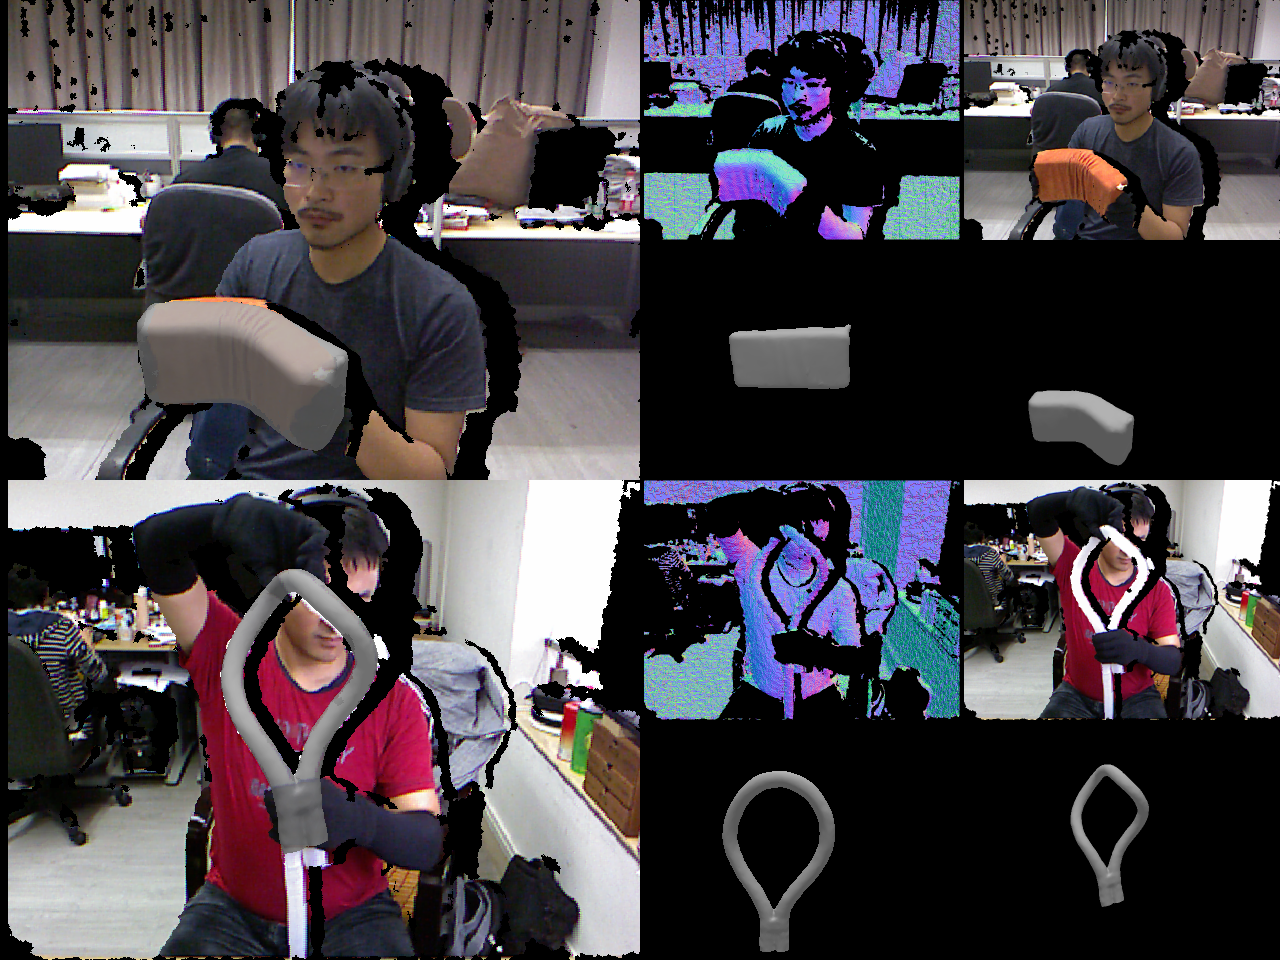
\includegraphics[width = \textwidth]{./Pictures/ds_p_t.png}
    \caption{样例pillow和tube的形变捕捉结果}
    \label{ds_p_t}
\end{figure}

本文采用了通用的形变描述方式,
并不需要形变的物体属于特定的类型,
如人手、人脸等。
因此本文能够捕捉大部分柔性物体的形变。
本文会从捕捉到的形变模型中挑选出部分有代表性的形变状态作为用于构建形变子空间的形变关键帧。
这些关键帧都会根据手部覆盖的区域对齐,消除冗余的刚体变换分量。
样例giraffe的形变关键帧,
以及对齐的结果以及在图\ref{before_after_align}和图\ref{align_area}中展示,
图\ref{pillow_tube_keyframe}展示了样例pillow和tube的形变关键帧和对齐后的结果。
第一行为pillow提取关键帧的结果,
第二行为tube提取关键帧的结果;
每行的第一张为未形变的模型,
最后一张为形变关键帧对齐的结果,
图中红色的部分为模型中用于对齐的部分。
形变捕捉的过程用没有用到特定类型物体的先验知识,
giraffe为长颈鹿形的毛绒玩具,pillow为小枕头,tube为塑料水管,
它们的形变都能很好的被捕捉。
而在对齐之后,本文消除了关键帧中整体偏移,
保证了由此构建出的形变子空间更加准确。

在之前的基于样例形变方法中,
样例都是人工编辑而成,耗费人力和时间。
而且对于现实中存在的物体,
人工编辑的形变样例也不一定满足物体本身的形变特性。
本文的所有形变关键帧全部通过捕捉物体在现实世界中的形变得到,
保证了形变关键帧的准确性。
\begin{figure}
    \centering
    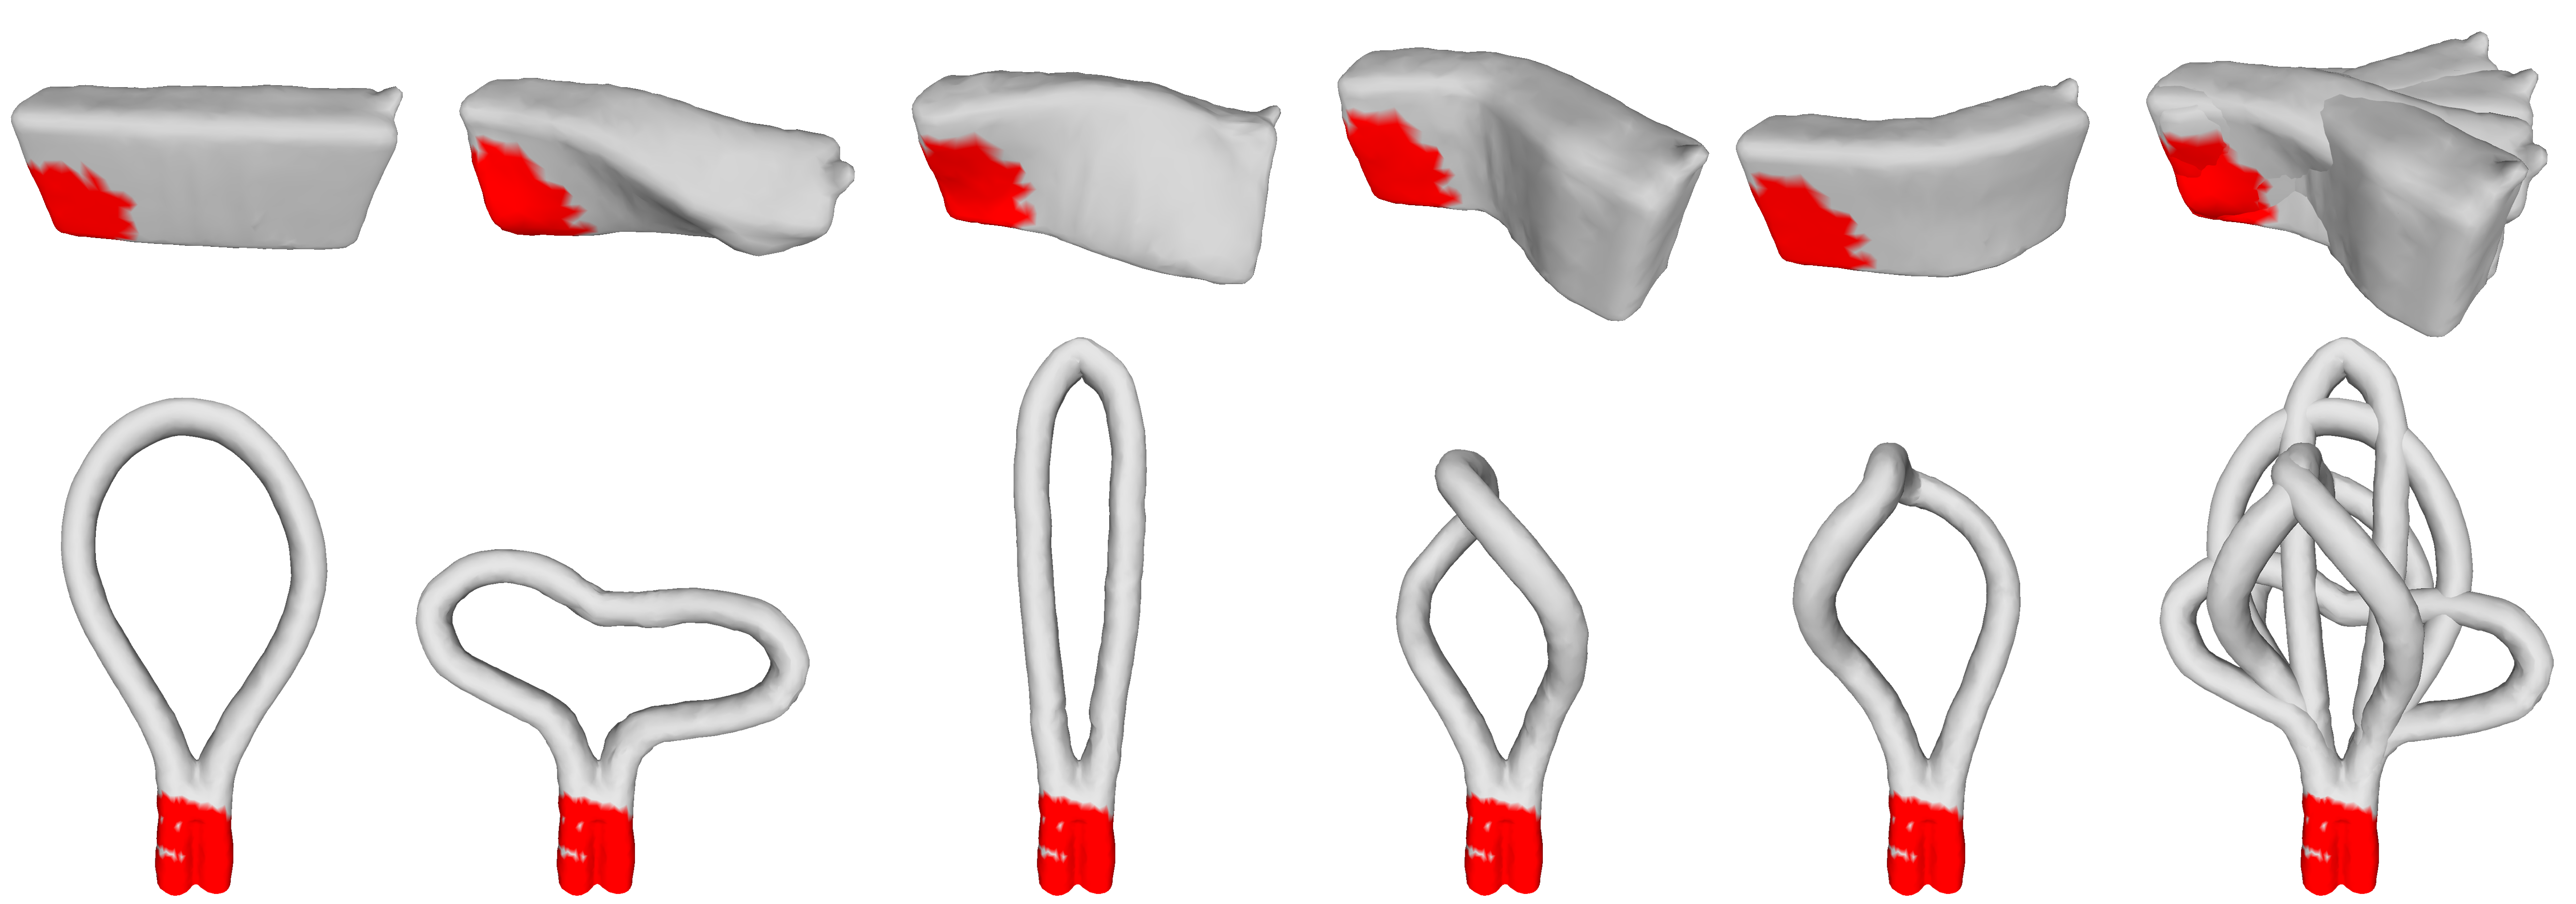
\includegraphics[width = \textwidth]{./Pictures/pillow_tube_keyframe.png}
    \caption{提取出的形变关键帧}
    \label{pillow_tube_keyframe}
\end{figure}

\section{形变子空间形变结果}\label{sec_subspace_res}
本文从形变图关键帧中提取特征向量,
特征向量描述的是形变模型相对初始模型的相对形变,
它由每个面片的形变形变梯度,即仿射变换中的非平移部分组成。
当对特征向量做插值并不是直接插值顶点的位置,
而是插值面片的变换。
所以本文中的特征向量插值不仅可以内插($0 \leq w \leq 1$),
在外插($w<0$或$w>1$)时依然能得到较好的结果。
图\ref{extrapolation}展示了各个样例上做内插和外插的结果。
图中的每一列分别为插值权重$w$的值分别为1.3、1、0.5、0、-0.5、-1、-1.3时的插值结果。
其中$w=0$时的模型为初始模型,
$w=1$时的模型为该特征向量对应的形变关键帧。
可以看出特征向量无论是内插还是外插,
甚至在权重为负数时仍然能得到自然的插值结果。
\begin{figure}[h]
    \centering
    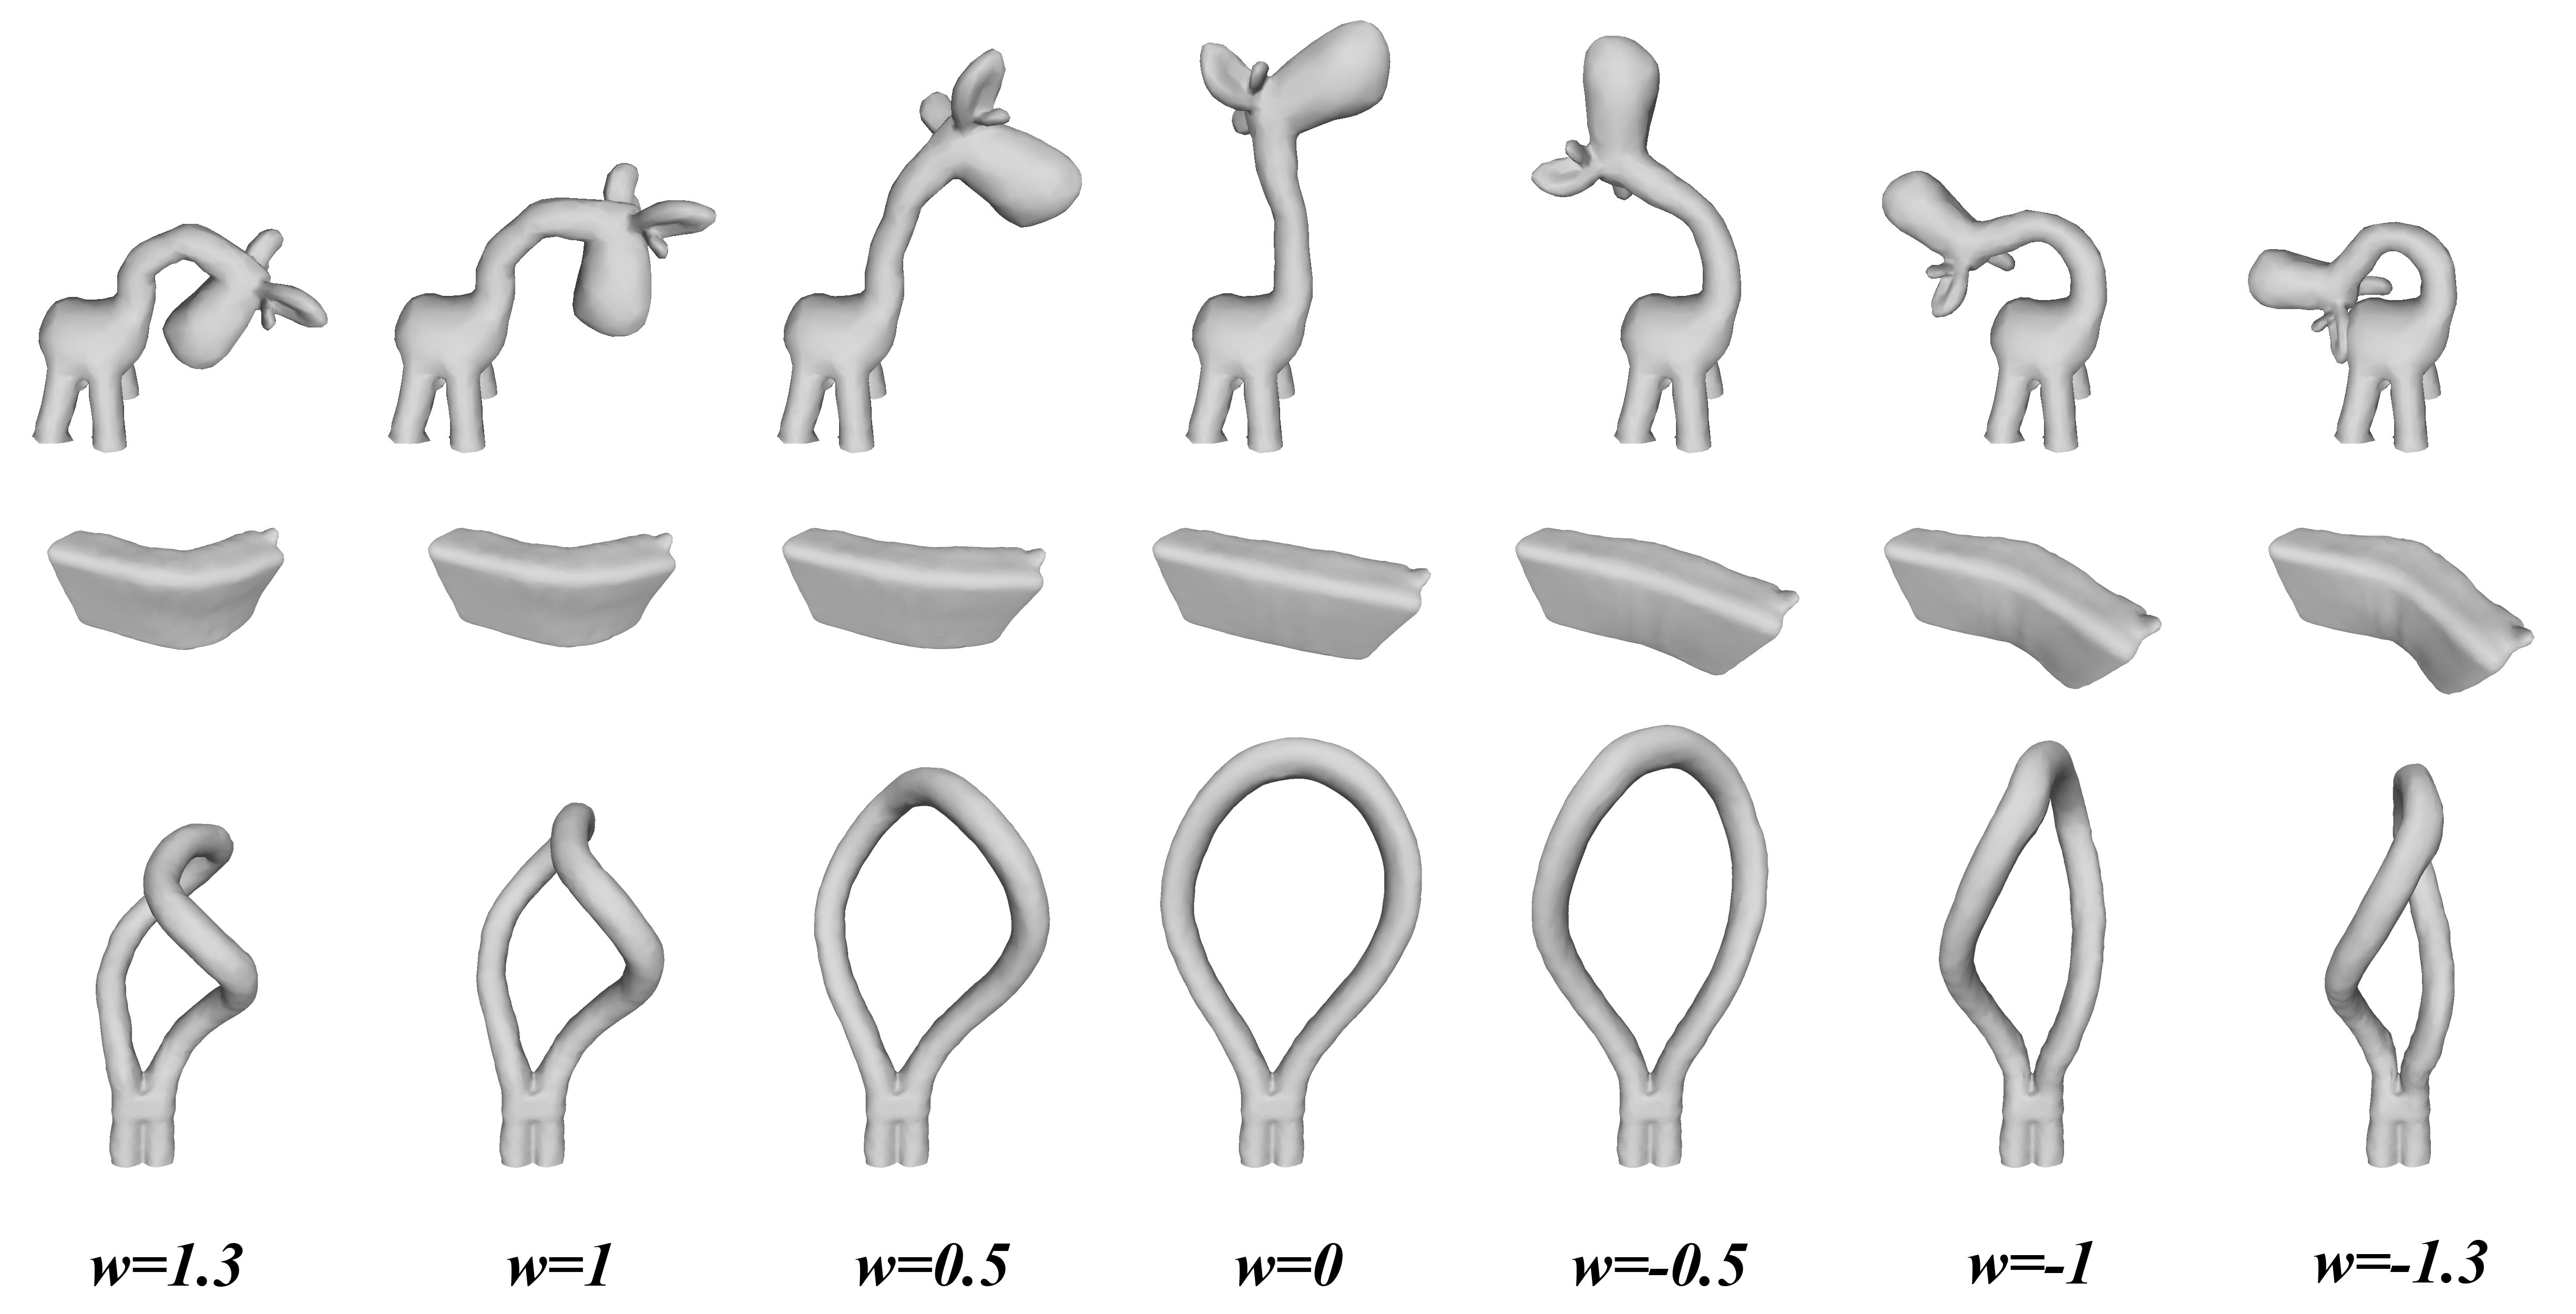
\includegraphics[width = \textwidth]{./Pictures/extrapolation.png}
    \caption{各模型上内插与外插的结果}
    \label{extrapolation}
\end{figure}

在基于形变子空间的模型修改方法里,
能量函数中的系数$\lambda_c$的值决定控制点的目标位置在形状修改时的权重。
当控制点仍然落在形变子空间内时,
$\lambda_c$的值对形变的结果并无明显的影响。
但当控制点被用户拖动到模型的形变子空间外的时候,
$\lambda_c$的值就决定了形状修改时的倾向。
图\ref{different_lambda}展示了$\lambda_c$取值不同时形状修改的结果。
图中位于模型头部的控制点被用户拖动到了形变空间之外的位置,
五张图从左至右分别为$\lambda_c$的值为1、10、50、100时形状修改的结果。
可以看出$\lambda_c$的值较小值,
形变修改的结果更倾向于让模型的形状落在模型的形变子空间内;
当$\lambda_c$的值较大的时候,
形变修改的结果更倾向于与让模型的形状更接近控制点。
图\ref{edit_result}展示了利用形变子空间形状修改得到的形变模型,
每幅图片下方的向量为各基向量的插值权重。
可以看出基于形变子空间的形状修改可以得到复杂而自然的形变结果。
\begin{figure}
    \centering
    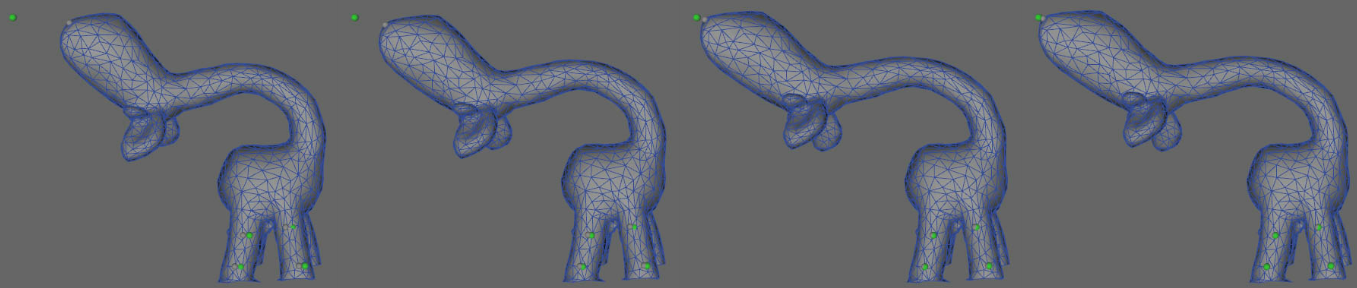
\includegraphics[width = 0.85\textwidth]{./Pictures/different_lambda.png}
    \caption{$\lambda_c=1/10/50/100$时形状修改的结果}
    \label{different_lambda}
\end{figure}
\begin{figure}
    \centering
    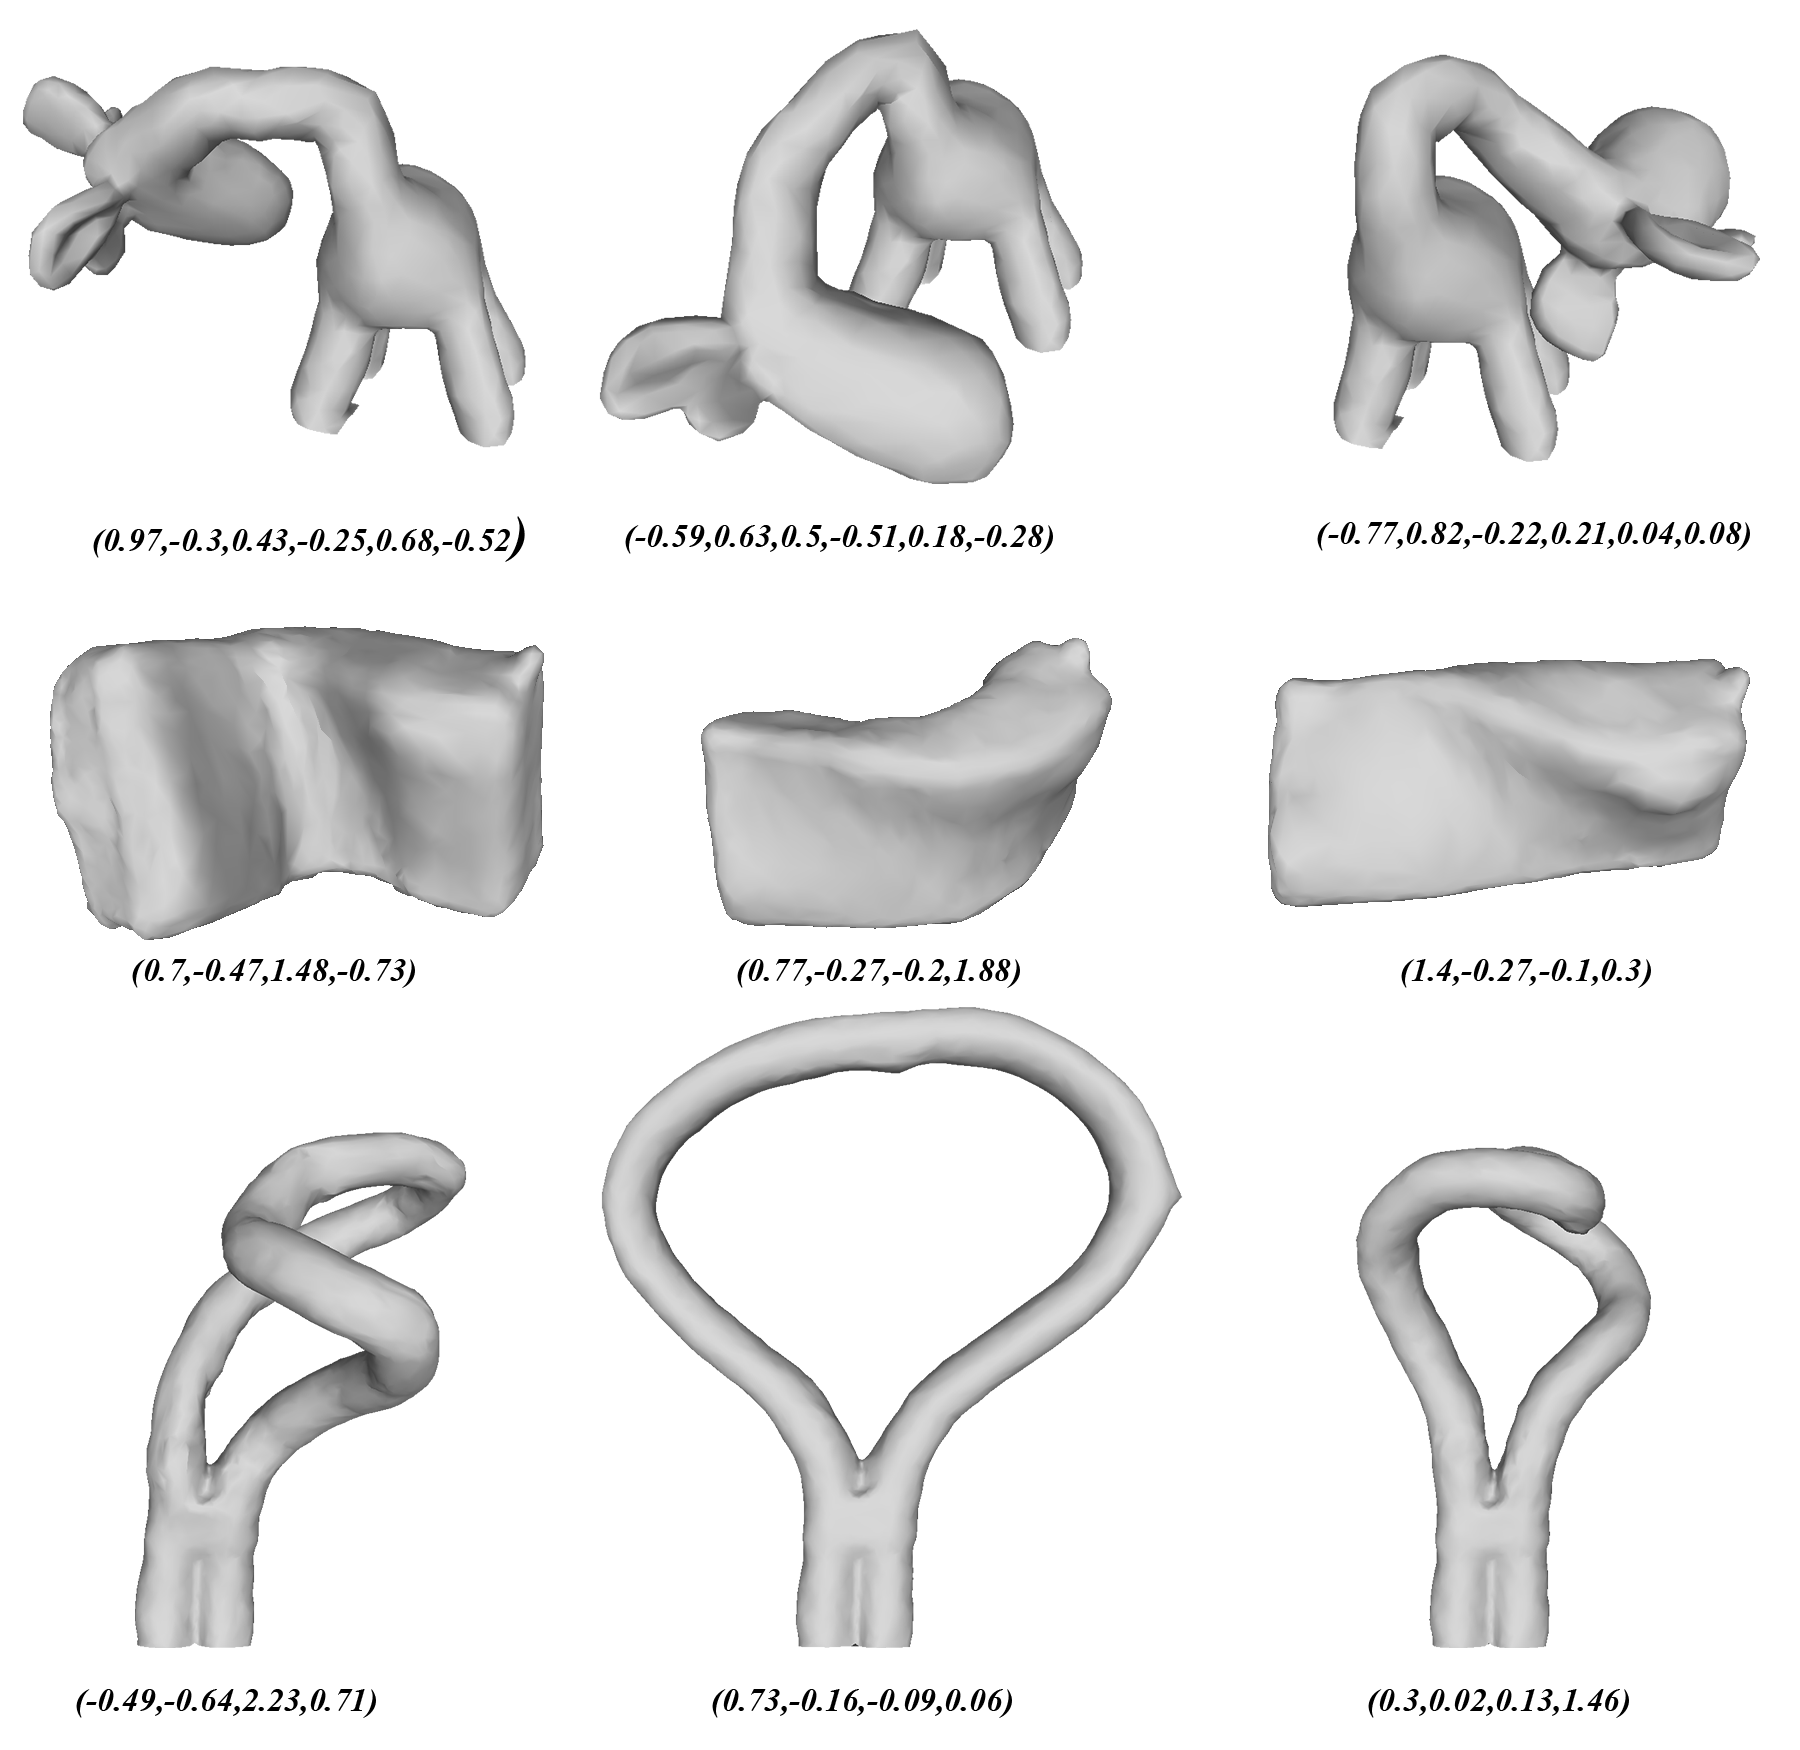
\includegraphics[width = 0.85\textwidth]{./Pictures/edit_result.png}
    \caption{通过模型修改得到的形变模型}
    \label{edit_result}
\end{figure}
\section{本章小结}
本章展示了分析了本文的实验结果。
首先,本章展示了在不同位姿下位姿估计算法的结果,以及位姿估计各阶段的耗时;
然后,本章展示了更多提取形变关键帧的结果;
最后,本章展示了特征向量的插值效果以及形变子空间形状修改的结果。

\chapter{总结与展望}
模型形状的修改在工业界有着广泛的应用。
本文提出了一个以RGBD视频为输入,从模型重建、形变捕捉到形变子空间构建的算法,
并给出了基于子空间的模型形状修改方法。
由于本文的模型通过扫描重建,
用于构建子空间的形变关键帧由形变捕捉得到,
形变关键帧一定是现实中物体会发生的,
所以由此构建的形变子空间是较为符合物体本身形变的特性的。

本文的算法也有着一些限制和可以进一步改进的方案。
首先,由于本文在形变捕捉阶段使用的形变描述方法会根据相邻节点约束传递形变,
本文的方法适合能捕捉平滑的柔性形变。
对于一些不连续的突变的形变,就不能很好的处理,如铰接件、抽屉等。
对于这种情况,不能用通用的柔性形变模型描述,
可以将模型分割为多个发生刚体变换的部分再各自跟踪各自发生的变换。

此外,本文的形变捕捉流程不能捕捉细微的形变。
这是因为本文形变捕捉方法中,
顶点的变换由形变图节点的形变插值而成,
又有相邻节点间的约束,
所以这种形变的描述方式描述不了局部的细小形变,
如物体表面的褶皱。
此外,本文使用的Kinect一代深度相机采集的深度数据精度较低且有较大的噪声,
无法准确捕捉物体表面的细小形变。
如需捕捉这些细小的形变,
可以使用精度更高的深度相机采集物体表面的深度信息。
此外可以用基于形变图的形变捕捉方法捕捉方法物体的大致形变姿态,
在用直接优化局部顶点偏移的方法获取局部的细小形变。

最后,本文在形变捕捉阶段用于形变图描述形变,
但在形变子空间构建时用每个面片的形变梯度描述模型的形变,
两个阶段描述形变的精度与形式不匹配。
针对这个问题有两个角度的改进策略。
一是在形变捕捉阶段,可以用更底层的方式,如顶点和面片的信息,描述形变。
二是直接根据形变图提取形变特征向量,构架基于形变图的形变子空间。

在未来的工作中,我们希望能够进一步拓展算法,
使之可以应用于更广泛的使用场景,
并用有高质量的结果。

\ZJUbackmatter
%%%%%%%%%%%%%%%%%%%%%%%%%%%%%%
%% 参考文献
%%%%%%%%%%%%%%%%%%%%%%%%%%%%%%
\ZJUthesisbib{mybib}

%%%%%%%%%%%%%%%%%%%%%%%%%%%%%
% 致谢页
%%%%%%%%%%%%%%%%%%%%%%%%%%%%%
\begin{thanks}
% 光阴似箭,我在浙江大学的求学生涯以及接近尾声。
% 在这几年中,我经历了很多,学习了很多,收获了很多,也成长了很多。

% 首先我要感谢我的父母和其他关心我的家人,
% 使他们无怨无悔的付出和全心全意的支持让我没有后顾之忧,
% 能够专心学业与科研。

% 衷心感谢我的导师侯启明副教授、周昆教师和郑友怡老师对我的悉心指导。
% 他们不仅授予我丰富的知识,
% 还培养了我良好的工作科研的习惯与态度。
% 他们在科研上严格的要求,严谨的治学态度和深厚的学术造诣一直在我求学的道路上指引着我。

% 由衷感谢实验室的所有同学们。
% 是他们的陪伴让我的研究生生活充满斑斓的色彩;
% 是他们的帮助帮我解决了学习中科研中遇到的众多问题。

% 最后我要感谢所有评阅论文和答辩委员会的各位老师,
% 感谢你们在百忙之中给予我指导。
由于论文送审需要,隐去本章节。
\end{thanks}


%%%%%%%%%%%%%%%%%%%%%%%%%%%%%%
%% 附录
%%%%%%%%%%%%%%%%%%%%%%%%%%%%%%
%\appendix
%\chapter{附录A}

这是附录A的内容。

\chapter{附录B}

这是附录B的内容。


%%%%%%%%%%%%%%%%%%%%%%%%%%%%%%
%% 索引
%%%%%%%%%%%%%%%%%%%%%%%%%%%%%%
%\ZJUindex

%%%%%%%%%%%%%%%%%%%%%%%%%%%%%%
%% 个人简历
%%%%%%%%%%%%%%%%%%%%%%%%%%%%%%
\begin{resume}
\begin{enumerate}
\item{第一条的内容}
\item{第二条内容}
\end{enumerate}
\end{resume}


%%%%%%%%%%%%%%%%%%%%%%%%%%%%%%
%% 发表论文目录
%%%%%%%%%%%%%%%%%%%%%%%%%%%%%%
%\begin{publications}
\begin{enumerate}
\item{第一篇}
\item{第二篇}
\end{enumerate}
\end{publications}


\end{document}
